\documentclass{article}
\usepackage[a4paper, tmargin=1in, bmargin=1in]{geometry}
\usepackage[utf8]{inputenc}
\usepackage{graphicx}
\usepackage{parskip}
\usepackage{pdflscape}
\usepackage{listings}
\usepackage{enumitem}
%%\usepackage[normalem]{ulem}
\usepackage{mathtools}
\usepackage{hyperref}
\usepackage{float}
% \usepackage{hyperref}
% \usepackage{titlesec}
\usepackage{caption}
\usepackage{subcaption}
%% To do:
% > Which led used
%% > Manchester Encoding ?


\newcommand{\ra}{$\rightarrow$}


\begin{document}


% \title{
\begin{titlepage}
   % \vspace*{\stretch{1.0}}
   \begin{center}
     \Large\textbf{EE 344 Final Report \\Visible Light Communication using LED}\\
     \vspace{3cm}
     \large \textbf{Group No. B-05}\\
     \large\textit{Arka Sadhu - 140070011\\Sudeep Salgia - 14D070011\\Parth Kothari - 14D070019\\}
     \vspace{3cm}
     \large\textbf{Faculty Mentor : Prof. Kumar Appiah}\\
     \large\textbf{RA associated : Akshay}\\
     \vspace{5cm}
     
\includegraphics[scale=0.15]{images/iitblogo}
   \end{center}
   % \vspace*{\stretch{2.0}}
\end{titlepage}

% Faculty Incharge: Prof. Kumar Appaiah\\
% TA Associated : \\
% Group Members:\\
% \author{
% \hline
% \maketitle
\newpage
\section{Abstract}
With the advent of technological developments in the Mobile web access and rapid increase in demand there has been a shortage of available spectrum. Traditionally communication has been done using radio waves, and due to this shortage there is an increasing need to look for different avenues and means for communication and therefore communication using visible light spectrum is a very promising prospect to address the situation. 

LiFi (Light Fidelity) is the new buzzword in new era of communication. It is often used to describe high speed Visible Light Communication (VLC). VLC dedicates itself to solving the problem of illumination and communication together. The way it is implemented is that the
light source is switched on and off at a very high speed, such that it is not discernible to the human eye, but a sensitive photodiode can detect it. This solves the problem of illumination and at the same we can encode information in the switching pattern and hence enabling us to transmit data, and recover it using the photodiode receiver. In our project, we aim to develop a prototype of Visible Light Based Communication link. The project consists of a transmitter, a LED in this case, which transmits the message signal which is received by the receiver.

\newpage
\tableofcontents
\newpage
\section{Chapter 1 : Introduction}
% Give Project objective, Block diagram, Motivation for the work
\subsection{Project Objective}
The project aims at developing a prototype to establish a commununication link which uses the visible spectrum for transmission. This is popularly known as Visible Light Communication (VLC). In addition, it seeks to balance the inherent trade-off between speed and distance with respect to accuracy. The final aim is to reach data rates of 1Mbps at 50cm with accuracy over 99\%.
\subsection{Block Diagram}
\begin{figure}[h]
  \centering
  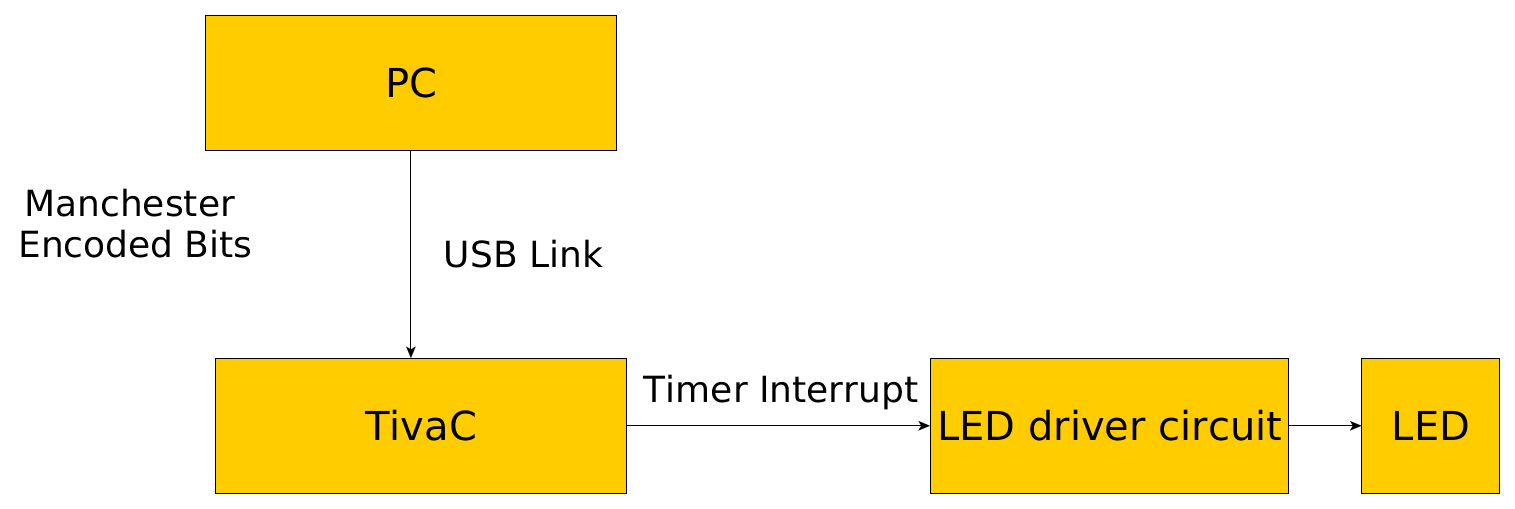
\includegraphics[scale=0.25]{images/tx_bd}
  \caption{Transmitter Block Diagram}
  \label{fig:1}
\end{figure}
\vspace{1cm}
\begin{figure}[h]
  \centering
  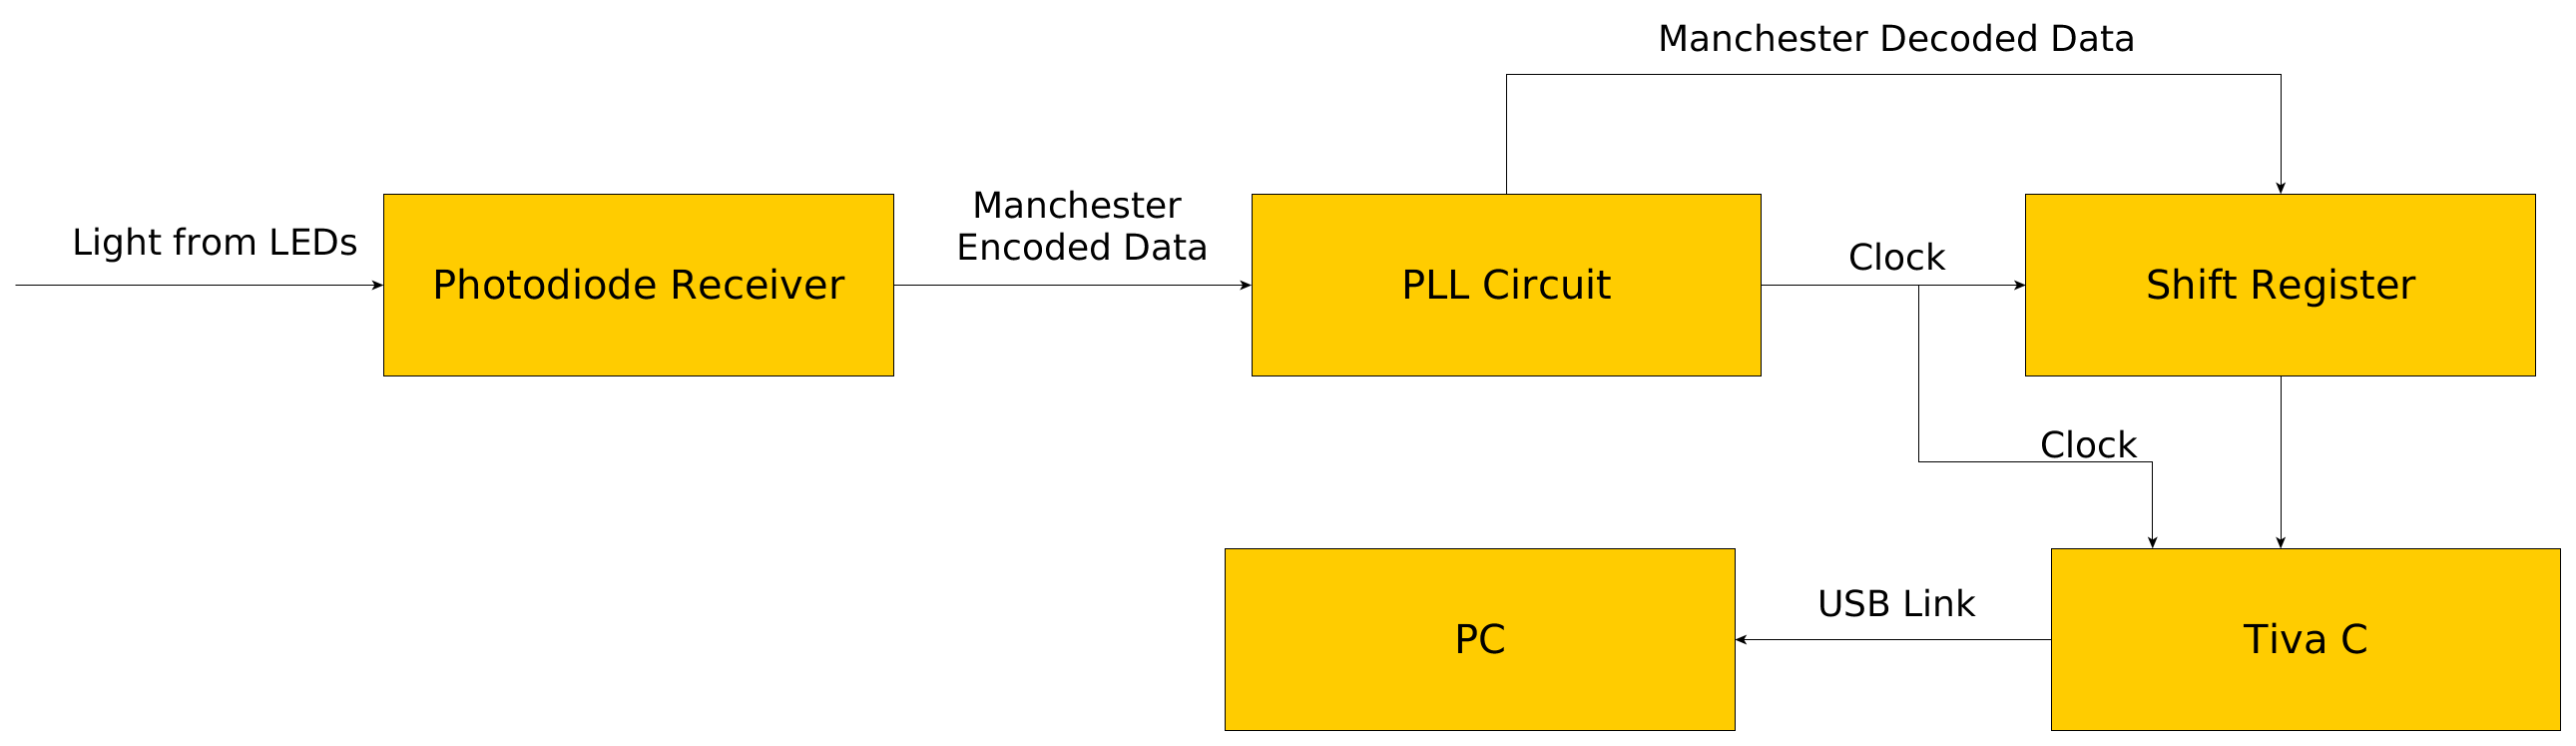
\includegraphics[scale=0.18]{images/rx_bd}
  \caption{Receiver Block Diagram}
  \label{fig:2}
\end{figure}
\subsection{Motivation for the Work}
Mark Twain had once remarked, “Buy land -- they’re not making it anymore”. Interestingly, in today’s context this holds even for the spectrum. With the spectrum limited anyway and its increased demand greatly driven by the need of the newer technologies like Internet of Things, there is an urgent need to look for solution of this spectrum-crunch. 
Surprisingly, the one plausible solution is staring right at us - visible light! This idea has led to a whole new fast developing field of light fidelity or popularly known as, LiFi. It is a term often used in place of Visible Light Communication which is a technique that aims at solving the problem of illumination and communication together. It achieves this by switching the light sources at high frequencies, making it indiscernible to the human eye by measurable by a sensitive photodiode. The applications of such a communication systems are numerous. Imagine the headlights of a driverless car communicating with the traffic lights in order to determine whether to move forward or not. Or take the case of indoor positioning position system, where the camera of the mobile can be used to communicate with the surrounding lights in order to determine our position in, say a large shopping.    
Thrilled by these varied applications, we decided to develop a prototype of Visible Light Based Communication link. The aim of this project is to send the data as fast as possible while maintaining a desired accuracy of reception. The project consists of a transmitter, a LED in this case, which will transmit the message signal which will be received by the receiver. The data transmitted would be read from a file.

\section{Chapter 2 : Project Design}
% Give details of the system design, choice of sub systems and other design
% steps/strateg
The design of project is aimed at establishing a communication link using the visible light where the data is taken from a file, sent over the link and again stored in a file at the receiving end. The challenge is not only in designing the hardware and the software systems individually but also design and implement a seamless integration between the two. In terms of hardware, a typical communication system has two parts, one each on the transmission and the reception end. Also to ensure synchronous transmission of data, the complexity of the receiver increases. Thus keeping in mind the above broad categorizations, the Hardware Module of the Project essentially consists of 4 sub systems, namely:
\begin{itemize}
\item The Transmitter Circuit
\item The Receiver Circuit
\item The Clock Synchronisation Circuit
% \item The Power Supply
\end{itemize}

The second and the third part together form the hardware at the receiver while the fourth system is essentially added to make the system portable.\\
The transmitter circuit has to essentially take the input data and send it over the link. The receiver circuit is designed to capture the data from the link and filter and process the waveform. The clock synchronisation part,as the name suggests, enable the synchronous reception of data by recovering the clock. For the ease of understanding, the Clock Synchronisation Circuit can further be sub-divided into
\begin{itemize}
\item Differentiator
\item PLL
\item Manchester Decoder
\end{itemize}

In addition to this hardware part,  we have a software part. At the transmission end, the data from a file is read into the tivaC board, where the data is encoded using Manchester encoding, and then sent out on a pin at the required frequency. The output of this pin is serves as the input to the transmitter circuit.

At the receiving end, the hardware itself does the decoding and hence it is just required for the tivaC to read the data and collect it and send it over the USB link to the computer at the receiving end. A shift register is used so that four pins can be read simultaneously. A protocol for starting and stopping the reception is also implemented. % The protocol and the shift register ensure that the bit error do not propagate. 

\subsection{Software Tools}
\subsubsection{Why TivaC}
We have used the board EK-TM4C123GXL TivaC (by Texas Instruments) for our project. Apart from its easy availability and being relatively cheap it has a wide array of features which were applicable to the project. It has an extremely fast processor and can work at speeds upto 80MHz (note: not instruction cycle). It has a large RAM of $32\text{KB}$ for data storage and $256\text{KB}$ for non-volatile storage which is extremely helpful especially for debugging purposes. It also easily supports the UART and we initially tested all our basic hardware using UART to ensure that there were no data loss at preliminary stages. Its main advantage is that it has support for PWM and USB Host functionality. The latter is extremely crucial for our project application. In total two TivaC have been used, one for Transmitter and another for Receiver.

\subsubsection{Why Code Composer Studio}
For all software coding and debugging purposes Code Composer Studio (CCS) has been used. CCSv7 (latest version) is an IDE for developing applicaitons on Texas Instruments (TI) embedded processors (like TivaC). There are a couple of other options like the Energia IDE, but there are quite a few advantages in using CCS. One of the most used feature of this IDE is the option for hardware debugging, which basically means that we can directly stop the code on a hardware breakpoint or a manual pause and stop. Also it is possible to have a look at Memory Map and all the current values of the variables at the breakpoint, save the current values to a file and a lot more. The main disadvantage if any would be the slightly steep initial learning curve but this is compensated by the extensive documentation and an extremely friendly and responsive online community. A few (difficult to remove) bugs are also mentioned in the report. 

\subsubsection{Communicating with the Serial Port}
There are two popular ways to communicate with the Serial port (though they are the same essentially). First, use a HyperTerminal or PuTTY or Cutecom any other similar client. With a clean gui, it can be directly used to communicate with the TivaC. Second, being using a python library. Two popular libraries would be PySerial and PyUSB. While this requires some knowlege of Python, it can pretty much be said to be self-content, in that with minimal learning, it can be used. Both methods have their merits and demerits. While the first one is extremely very easy to use, not much can be extended from it, and for applications like file transfer it is recommended to write the whole thing from scratch. Similarly for the second, it seems slightly daunting at first, but after knowing the pre-requisites, it can be effiiciently used for code debugging. For our purposes PySerial and PyUSB worked well.
\section{Chapter 3 : Project Implementation}
% Give details of the various subsystems (include neat circuit diagrams (no
% hand drawn diagrams please) with component values, photographs).
% Please do not give listing of your code in the report. Instead add
% comments to your code and upload it on YAWP (after the Final demo). We
% shall involve the TA/RA associated with your project for this step.
\subsection{Communication Protocol}
We have used On-Off Keying (OOK) along with Manchester encoding. On-Off keying is simply giving 5V output when bit is 1 and 0V output when input is 0. While On-Off Keying has the disadvantage of lessening the average value of the light and hence reducing the intensity, its simplicity of implementation and debugging were the primary motivations behind the choice.

Manchester Encoding simply encodes bit 1 as 10 and 0 as 01. The Manchester encoding on top off OOK naturally applies to the PLL circuit, and the PLL circuit directly gives us the manchester decoded output and this was our prime motivation for using this encoding.

For Transmission initially a sequence of 0s is sent, which when manchester encoded gives a sequence of 01, and helps in locking of the PLL. Then a start sequence is sent and then the actual data to be sent, and a terminating message. These sequences are known to both the Transmitter and the Reciever, and therefore the Reciever knows when to start saving the data and when to terminate. 

\subsection{Transmitter Code}
The job of the transmitter (TivaC) is to send manchester encoded bits to the Transmitter circuit periodically. While this seems to be a trivial task at first using a Timer Interrupt there are some problems especially because of the USB link. The TivaC has a USB receive buffer which gets filled when anything is sent from the PC. This transmission is achieved using Pyserial and PyUSB. When the TivaC receives data from the PC it immediately goes into the receive handler interrupt which then uses the received bits and stores it into its memory. This funcion disrupts the normal transmission using the Timer Interrupt and as a result the whole hardware goes hayway. There are also many other issues like the initial 30 bytes received by the TivaC are garbage value and there needs to be some buffer (3-4 seconds) between connecting the USB and sending the bits from PC. For testing purposes it is best to HardCode the file into TivaC, as mentioned the TivaC has a sufficiently large non-volatile memory.

Once what data is to be transmitted is known, the transmitter manchester encodes the data and stores it into a buffer. It initially sends a synchrnoising sequence which is used by the PLL for locking, and once the PLL is locked, it keeps on sending the data to be transmitted in a circular manner (implemented as a circular array). Few additional bits are also required for the synchronous circuit to work. A start sequence and end sequence are added at the start and end respectively to the data being transmitted. This helps the receiver in deciding when to actually start capturing the data bits. 
\subsection{The Transmitter Circuit}
The Transmitter circuit takes the data (to be sent) as the input from the TivaC board and drives the LED according to the input data. The circuit is a simple one comprising mainly a LED driver  and resistor to control the intensity of the light.

Our implementation of the circuit uses the IC SN7440N which is a dual quad input NAND gate to drive the signal. There are pull up resistors at the input and similarly pull down resistors at the output to control the amplitude of the driven signal and hence the average intensity of the LED.

This is an essential factor because often in VLC applications the primary application of the light source is not communication but rather is to provide illumination. Thus it is essential that we should not be affecting the primary purpose in order to achieve the dual motive. Another reason that necessitates control of average intensity is the sensitivity of the photodiode. Often the photodiode that is used is sensitive in a range of intensities and tends to underperform or saturate if we use it outside this range Thus depending on the distance between the transmitter and the receiver we might have to tune these values. For the LED driver any simple logic gate can be used with appropriate function. We have employed a NAND gate for the purpose because of its low resistance of the NAND gate when a low logic is driven at the output which ensures that the output is not affected.

\begin{figure}[h]
\begin{subfigure}[t]{0.5\textwidth}
	\centering
	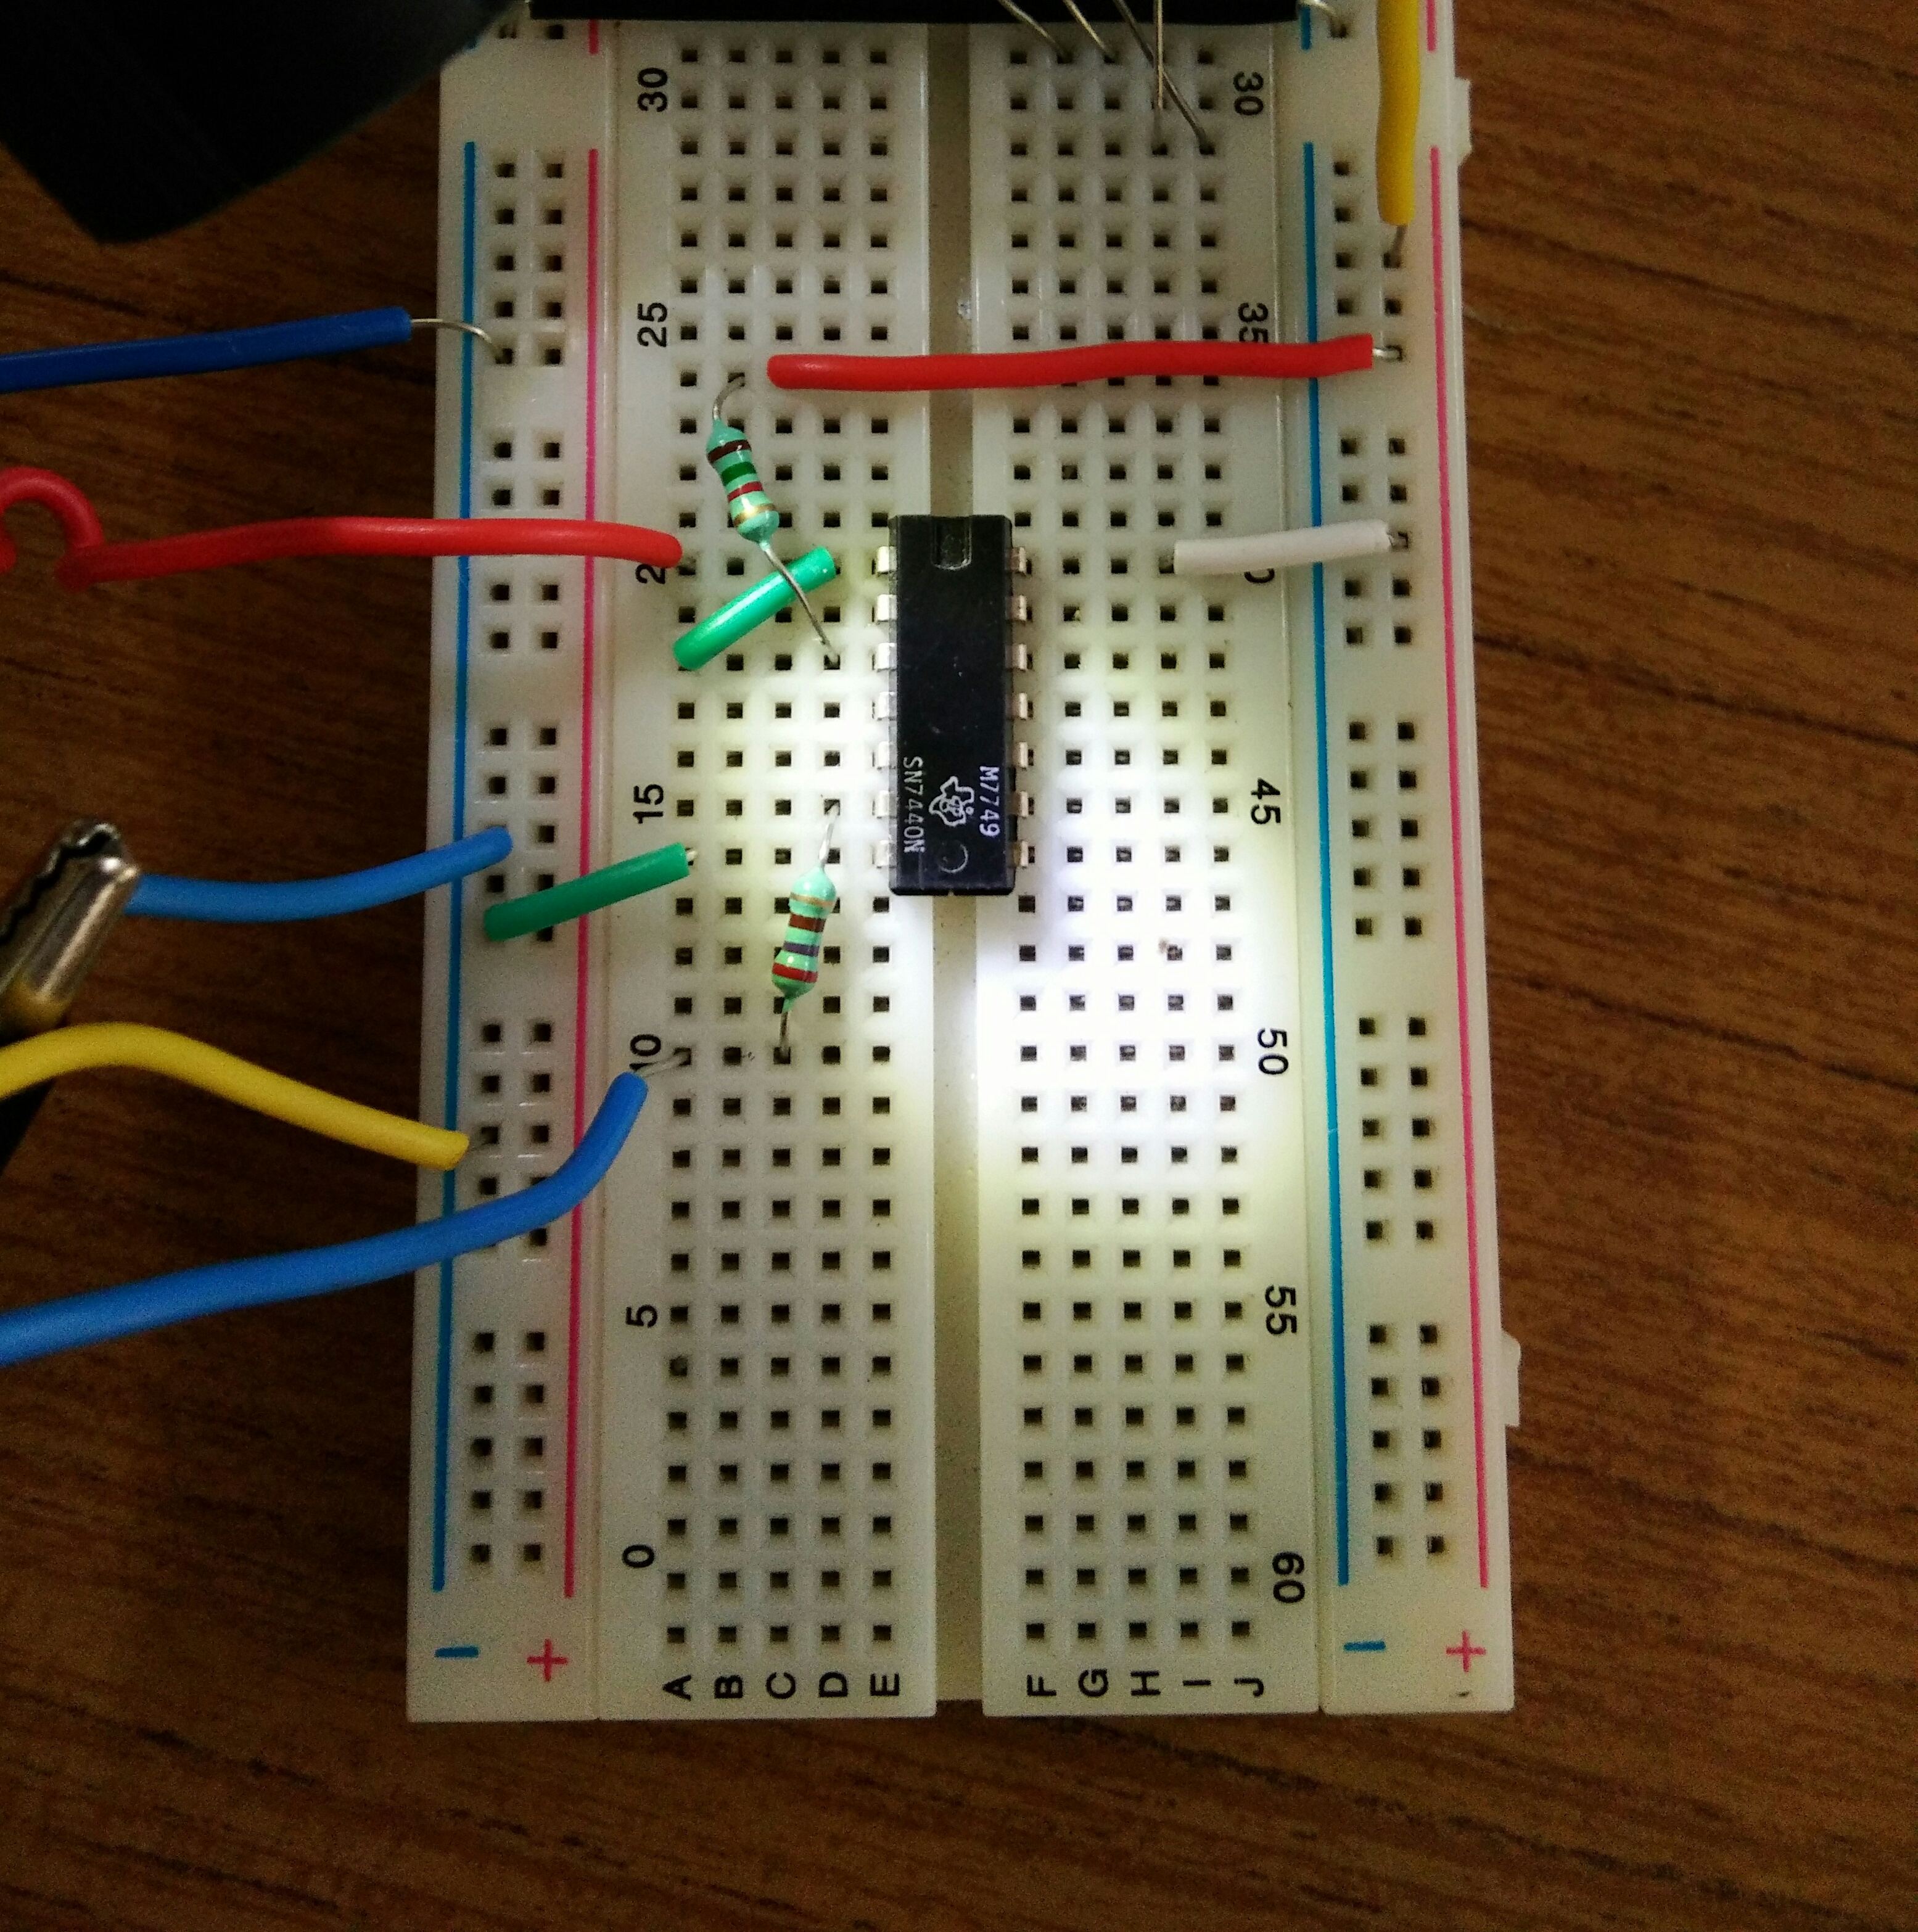
\includegraphics[scale = 0.1]{images/Transmitter.JPG}
	\caption{Transmitter implementation}
	\label{Fig :1b}
\end{subfigure}
% \begin{subfigure}[t]{0.5\textwidth}
% 	\centering
% 	\includegraphics[scale = 0.4]{noisy_30.jpg}
% 	\caption{Noisy image}
% 	\label{Fig :1b}
% \end{subfigure}
% ~

\end{figure}

%%%%%%%%%%%%%%%%%%%%%%%%%%%%%%%%% PICTURE%%%%%%%%%%%%%%%%%%%%%%%%%%%%%%%%%%%%%%%%%%%%%%%


\subsection{The Receiver Circuit}
The Receiver Circuit, as the name suggests, corresponds to the hardware at the receiving end of the signal that is used to capture the signal and retrieve it. In essence, this circuit captures the data, amplifies the captured signal, filters the noise to retrieve the waveform which can be used for clock synchronisation.

The light is captured by a photodiode which generates a current whose magnitude is proportional to the intensity of the light falling on the photodiode. It is essential to note that there is a range of intensities where the performance of photodiode is good and it should be ensured that the diode is operated in this range so that output is not saturated.

Our implementation of the circuit uses BPW34 photodiode for this purpose. One of the main reasons to use this was because this had a reasonably small fall and rise time of about $100ns$ which would enable us to operate at higher frequency ranges to quickly switch data enabling better data rates. The photodiode gives a very small current of the order of microamperes$(10^{-6}\text{A})$ which has to be amplified before using it. Hence the current is passed through a large resistor to amplify the voltage which is connected to a voltage buffer to further use this voltage. The buffer ensures isolation of the remaining part of the circuit the above. This is essential because the current in this part of the circuit is very low which might get affected by the other parts in the circuit if it were to be connected directly.

The buffer is made using a standard OPAMP implementation of the same by using a TL082. The OPAMP also support high switching rates and thus must have a high slew rate so that the data does not get affected. With a slew rate of $13V/us$ TL082 was a good choice for the purpose. The received waveform is corrupted with noise which has to be filtered out.

Interestingly, this application does not have a noise in the high frequency range but instead has in the low frequency range. This is primarily because the noise added to the system comes from the ambient light falling on the photodiode. The fluctuations in the intensity have a frequency component equal to that of frequency of the supply equal to 50Hz. Thus it is essential to remove the 50Hz component from the received signal. If this not done, then the waveform looks like a actual one modulated on a very low frequency wave (which actually corresponds to the 50 Hz).  Thus the waveform is passed through a simple RC high pass filter with a cutoff frequency of $700 Hz$.

The waveform at this point has been affected and loses it rectangular shape. To ensure recovery of the original rectangular waveform, the output is passed through a comparator. The comparator used here is LM361 which works very well upto $1 MHz$ which is well above the required range. The output of the comparator is then fed to the clock synchronisation and frequency correction circuit.


\begin{figure}[h]
\begin{subfigure}[t]{0.5\textwidth}
	\centering
	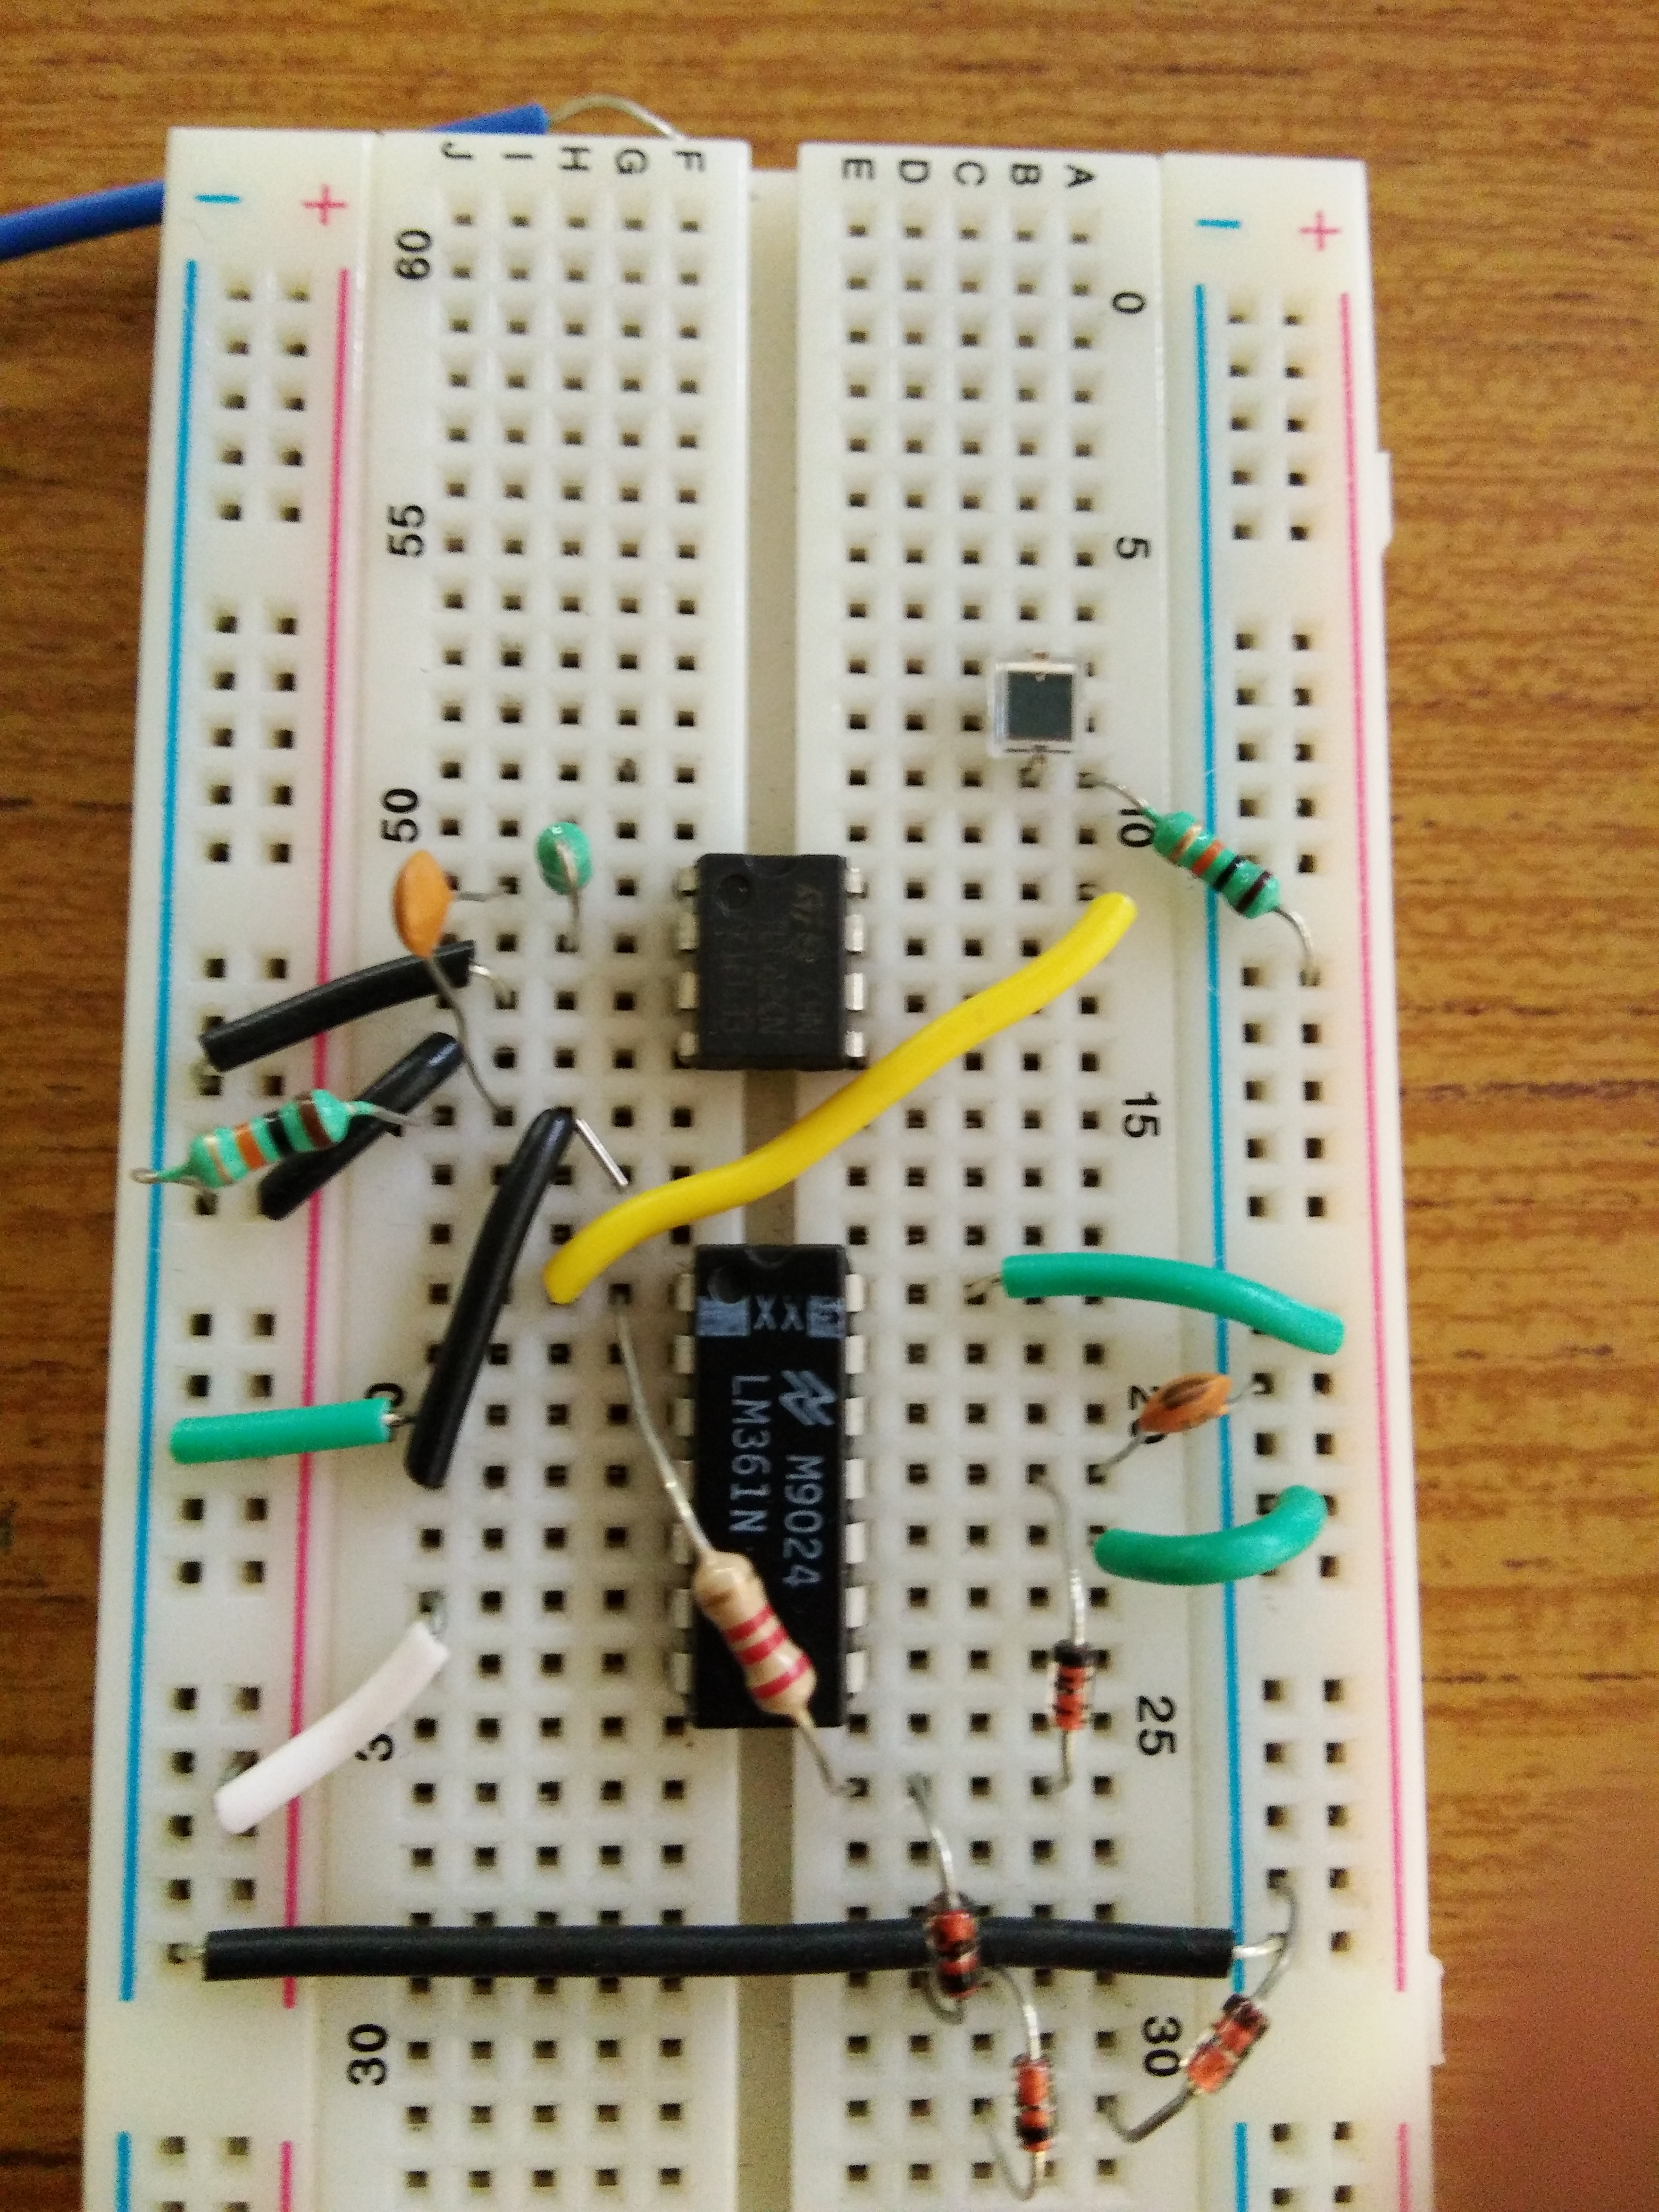
\includegraphics[scale = 0.1]{images/Receiver.jpg}
	\caption{Receiver implementation}
	\label{Fig :1b}
\end{subfigure}
~
% \begin{subfigure}[t]{0.5\textwidth}
% 	\centering
% 	\includegraphics[scale = 0.4]{noisy_30.jpg}
% 	\caption{Noisy image}
% 	\label{Fig :1b}
% \end{subfigure}
% ~

\end{figure}

%%%%%%%%%%%%%%%%%%%%%%%%%%%%%%%%%PICTURE%%%%%%%%%%%%%%%%%%%%%%%%%%%%%%%%%%%%%%%%%%%%%%%

\subsection{The Clock Synchronisation and Frequency Correction Circuit}
The Clock Synchronisation and Frequency correction functions to extract the clock from the received signal and synchronize the extracted the clock with the received signal. This particular step is essential as we need to obtain a reference clock with respect to which  we will sample the received data. Not just that, the reference needs to be the aligned in such a manner such that correct sampling occurs, that is, the data is sampled at the correct instant.

The above circuit consists of 3 sub-circuits :
\begin{itemize}
\item \textbf{The Differentiator Circuit}
\item \textbf{The Phase Lock Loop (PLL) Circuit}
\item \textbf{The Decoder}
\end{itemize}
It is useful to discuss the working of the PLL circuit as it will help explain the working of the entire clock recovery and data decoding circuit.

\begin{enumerate}[label=(\Alph*)]
\item \textbf{The Working of PLL}\\
  The generic working of the PLL is explained in this section. The working specific to the Visible light communication application is explained in the next section. The PLL takes as input a signal, say Vi, with an input frequency fi which is then passed through a phase detector. A phase detector, basically a comparator, compares the input frequency fi with the feedback frequency fo coming out of a device called VCO (voltage controlled oscillator).The phase detector provides an output error voltage Ver (=fi+fo) and an approximately DC voltage (=fi-fo). This combination of signals is then passed on to an LPF. The LPF removes the high frequency noise and produces a steady DC level, Vf (=Fi-Fo). 
The DC level is then passed on to a VCO. The output frequency of the VCO (fo) is directly proportional to the input signal. Thus, more the difference in the frequencies, more the changes in comparator frequency brought about by the VCO. Both the input frequency and output frequency are compared and adjusted through feedback loops until the output frequency equals the input frequency. The frequency comparison stops as soon as the output frequency is adjusted to become equal to the input frequency. This stage is called the phase locked state. This property of PLL, of generating a frequency signal, referred to as the “clock”, equal to the frequency of data transmission will be used to sample the data and thus decode it correctly.

%%%%%%%%%%%%%%%%%%%%%TO BE Completed%%%%%%%%%%%%%%%%%%%
\item \textbf{The PLL Clock Synchronisation Step}\\
  It is necessary for the PLL to determine the rate at which the data is going to be sent to it in order to generate a clock to sample the data (as explained above). Hence, a sequences of 1’s and 0’s need to be sent to the PLL, before the actual data is sent, so that it can determine the clock at which data is being transmitted. This step is called the “Synchronisation Step”. 

The question which follows immediately is how does the PLL circuit remember the clock once the actual data starts getting transmitted. As mentioned earlier, the data sent and received will be Manchester encoded. And obviously, the data will be a sequence of 1’s and 0’s which will be aperiodic. The transitions from high to low can take place at any time depending on the data being sent. The PLL is not supposed to respond to EVERY transition but only to a selected number of transitions which are periodic and correspond to the actual frequency of the data sent. An example is shown below.

%%%%%%%%%%%%%%%%%%%%%%%%%%%%%%%%%%%%%%%%%%%%%%55% *PIC* %%%%%%%%%%%%%%%%%%%%%%%%%%%%%%%%%%%%%%%%%%%

\begin{figure}[h]

	\centering
	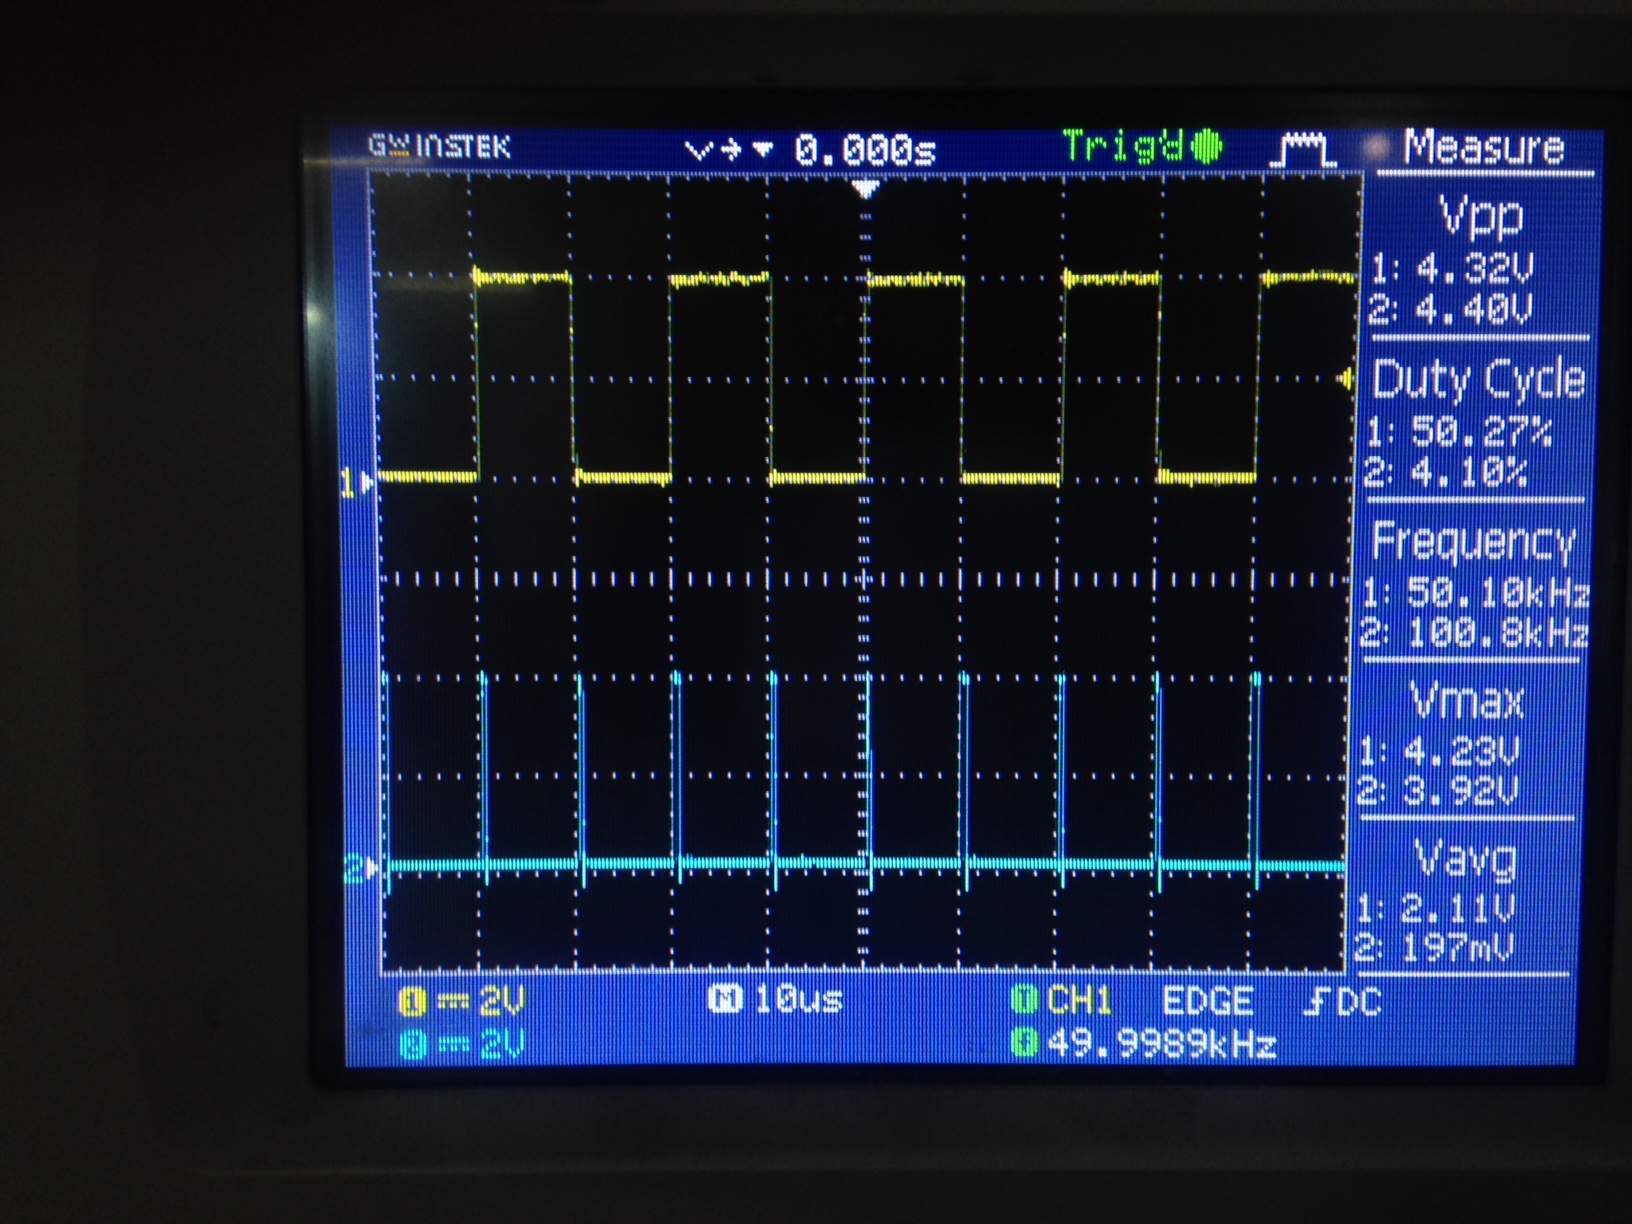
\includegraphics[scale = 0.1]{images/Diff_all_pulses.JPG}
	\caption{Differentiator showing pulses on each edge}
	\label{Fig :1b}


\end{figure}

As it can be seen in the picture shown above, if the differentiator captures every high to low transition, a waveform will be obtained which corresponds to the signal B. But the transitions, which corresponds to the actual clock, that is the ones which PLL actually needs to receive at its input are circled in the signal B. So the primary question is how to get rid off the unwanted the unwanted transitions?  
The answer lies in the special feature of PLL IC CD4046B called the Phase Comparator II

\item \textbf{The Phase Comparator II}\\
  Phase Comparator II is an edge controlled digital memory network. The comparator acts only on the positive edges of the data signals and comparator input signals. The duty cycle of signal and comparator inputs are, thus, NOT important. If the frequencies and phases of the input and output signal do not match, then the capacitor voltage increases or decreases correspondingly (according to the working of PLL explained above) such that the frequencies and phase become equal. The main point to be noted here is that Phase Comparator II has memory! During the ON intervals, that is when the pulse is present at the input of PLL, it provides the clock output as it should. But during the OFF intervals, that is the scenario where the pulse is NOT present at the desired time instant, the Phase Comparator II remembers the old clock and provides the previous clock output! This fact is utilized to remember the clock during the transition of moving from the synchronization pulse to the beginning of actual data transmission.

With the above knowledge, the working of the entire circuit can now be explained.

% \includegraphics[scale=0.5]{images/PLL_diagram}

\item \textbf{The Differentiator Circuit}\\
  As described in the phase comparator II section, the phase comparator II of the PLL responds only to the positive edges of the data input signal (or the comparator input signal). Thus, the differentiator is used in order to get pulses corresponding to the rising and the falling edges of the data. The reason for considering both the rising and falling edge transitions is that in the manchester encoded “0”, that is, half cycle low and half cycle high bit, the low to high transition corresponds to the actual clock signal to be extracted ( for example, the first and the third peak in signal B of the diagram) while in the manchester encoded “1”, that is, first half cycle high and next half cycle low bit, the high to low transition corresponds to the actual clock signal to be extracted ( for example, the fourth and the sixth peak in signal B of the diagram). Hence, differentiator is used to give pulses at both the edges.

\item \textbf{The PLL Circuit}\\
    \begin{figure}[h]
    % \centering
    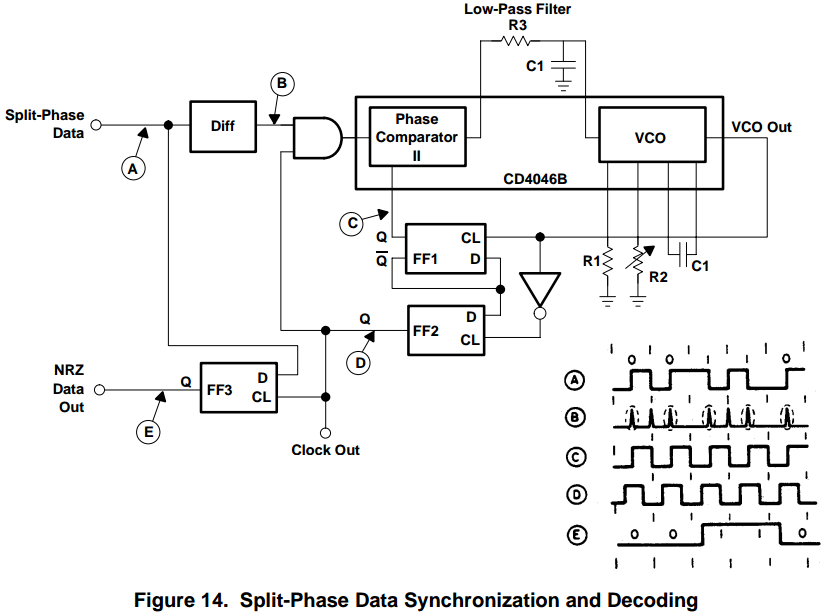
\includegraphics[scale=0.45]{images/PLL}
    \caption{PLL}
    \label{fig:PLL}
  \end{figure}

  The PLL Circuit consists of the IC 4046B, FF1 and FF2 as shown in the above diagram. The data signal input of PLL circuit is the output of the AND gate. Assuming that the input signal correspond to the pulses of the actual clock underlying of the data (reason to the provided later), the output of the VCO is a clock at twice the data frequency. The reason is that the VCO output is passed through the FF1 which divides the frequency of VCO output by 2. The output of FF1, which corresponds to signal C in the above diagram, is fed to the comparator input signal of PLL. Since locking takes place between the data input signal and comparator input signal, thus, the frequency of the comparator input should be same as that of data. And thus, the frequency of VCO output turns out to be twice the frequency of data because of the voltage divider present in between.

  The idea behind keeping a frequency divider after the VCO output revolves around the fact that the PLL circuit needs another signal, whose clock is 90 degrees phase shifted with the actual clock in order to select only those output pulses of the differentiator which correspond to the actual clock. See the signals B, C and D in the above figure together. B contains pulses at all those instants where a transition has taken place in the data signal. C has the same phase and frequency as the input signal. D is 90 degree shifted version of C. The question which remains to be answered is how does C correspond to the actual clock frequency and phase even after actual data has started transmitting?
  
The answer as described above is the magic of Phase Comparator II (PC II). When the transition took place from synchronising data to actual data, the PC II, remembered the old clock and continued to give the output C. Later, D being 90 degrees out of phase with C (precisely speaking, leading C), was “AND”ed with the output of the differentiator. Because of this, as shown in the above figure, only the pulses correspond to the actual clock survive! And thus, the PLL circuit still retains the actual clock frequency.    



\item \textbf{The Decoder Circuit}
  The decoder circuit decodes the manchester encoded signal on hardware itself. It consists of a single flip flop (FF3 in the figure) whose data input is the actual signal and clock input as signal D. As seen in the figure, the output of FF3 is signal E, which when sampled at the falling edges of signal D gives the desired manchester decoded data. 
  
\end{enumerate}

\begin{figure}[h]
	\centering
	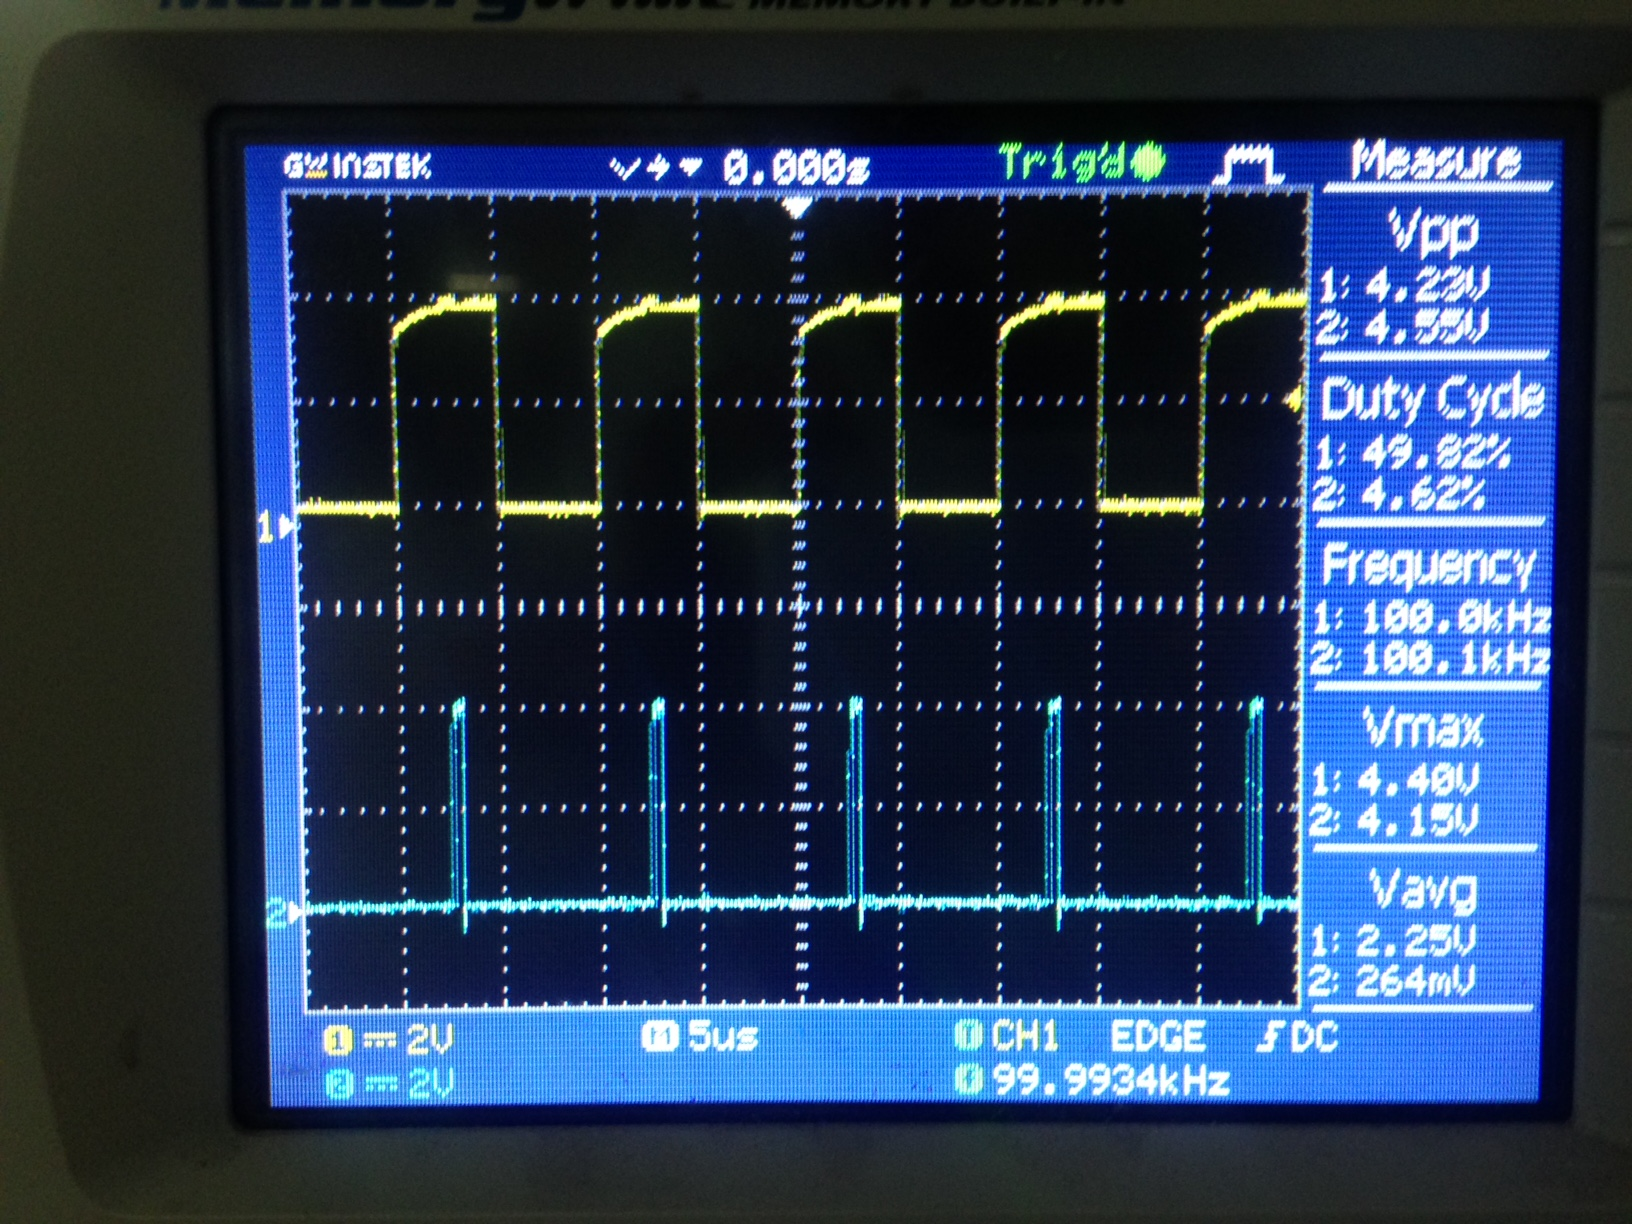
\includegraphics[scale = 0.1]{images/Diff_one_pulse.JPG}
	\caption{This is the pulse D with the input to the PLL}
	\label{Fig :1b}
\end{figure}

\begin{figure}[h]
	\centering
	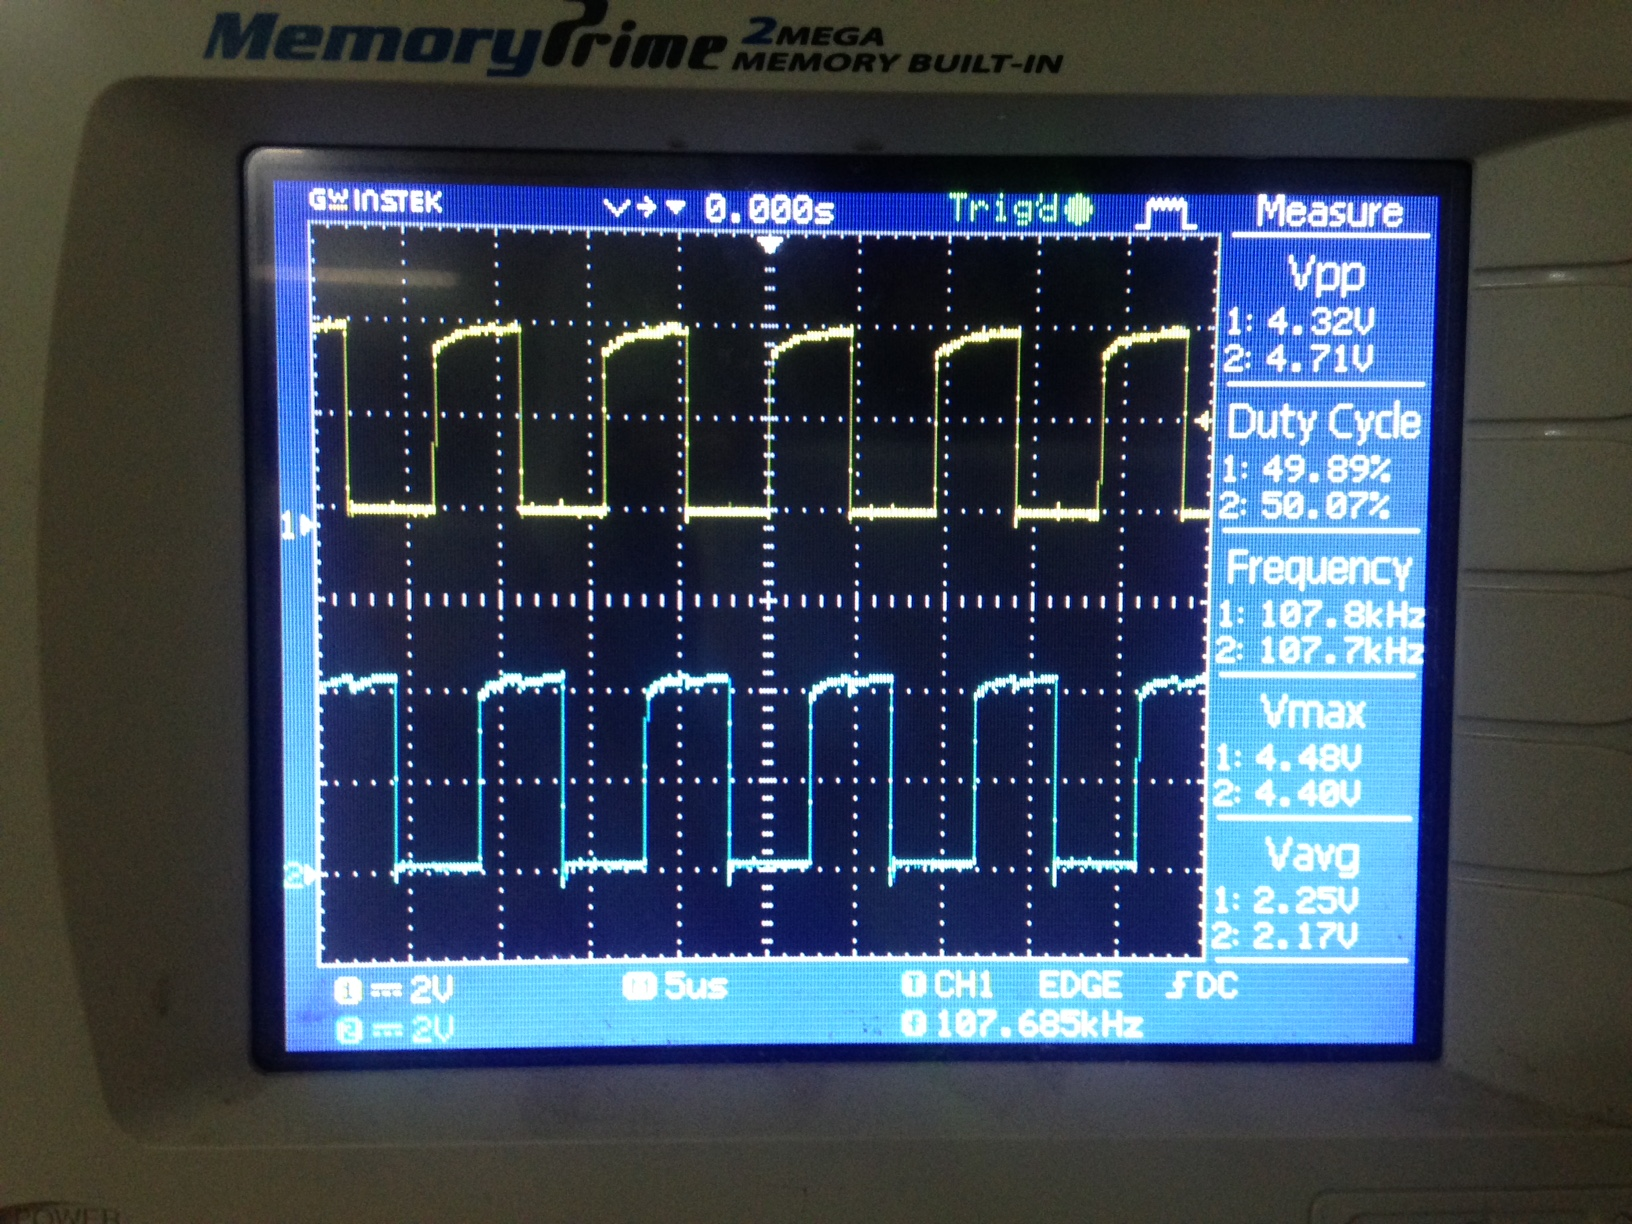
\includegraphics[scale = 0.1]{images/CD.JPG}
	\caption{The figure shows the $90^\circ$ phase difference between the C and D pulses}
	\label{Fig :1b}
\end{figure}

\begin{figure}[h]
	\centering
	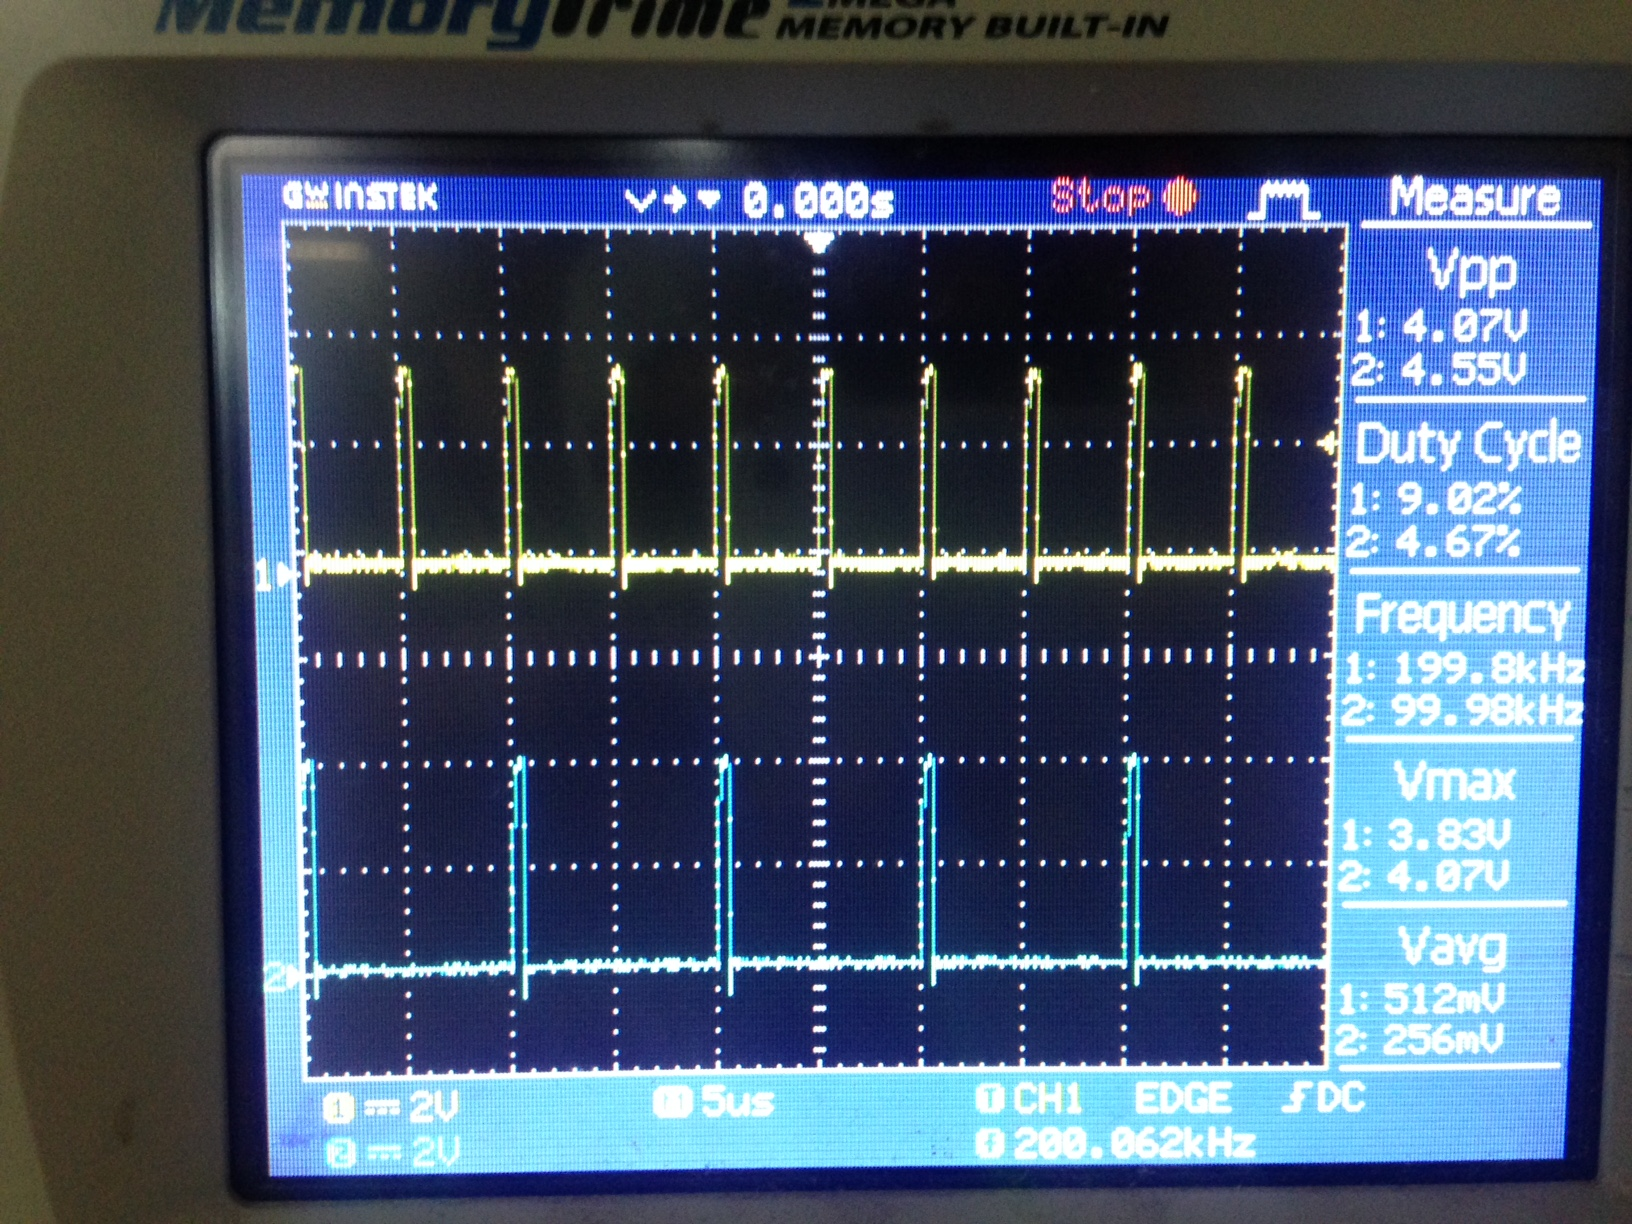
\includegraphics[scale = 0.1]{images/Selected_pulses.JPG}
	\caption{The figure shows the alternate pulses which have been captured}
	\label{Fig :1b}
\end{figure}

\subsection{Shift Register and Receiver Code}
The receiver circuits outputs the manchester decoded bits and the clock. This is passed through a shift register. We have chosen SN7495 as the shift register. 
\begin{enumerate}
\item \textbf{Shift Register}
  The shift register has many modes and for the project serial shift left and parallel load is used, i.e. it bascially takes in a serial input and gives parallel output on 4 pins. It takes the PLL clock and data output as its input and synchronously gives output the current 4 bits of the data.
\item \textbf{Receiever Code}
  The receiver has 4 pins from the shift register going into its 4 gpio pins. The clock is also sent to a gpio pin of the TivaC, and a gpio interrupt on this pin is initialized with the interrupt being called at the rising edge. When a rising edge is detected an interrupt function handler is called which then reads the 4 gpio pins to get the data of the shift register. 
  
  The receiver (TivaC) initially checks for a start sequence. When this start sequence is found it knows that anything after this will be valid data. Since the shift register gives 4 pin output, the reciever checks in multiples of 4 and uses those data for making up a whole byte. This is done with respect to the start sequence that is after every $4^{th}$ clock cycle it checks whether or not to read the data or not. Thus at every $(4k+1)$ rising edge it receives the lower nibble and at every $(4k)$ rising receives the higher nibble and combines them to form a byte and increments the array pointer.  

  At the same time it also checks if the end sequence has come. Once it sees the end sequence it disables the interrupt. Here also all the problems associated with the USB creep in. Hence we need to make sure that the USB interrupts are not enabled before everything is received.

  Once everything is received it sends the received data to the PC using USB link.
\end{enumerate}

% \subsection{Power Supply}
% To make this system portable another component has to be designed in addition to the above which is the power supply, one each for the transmitter and the receiver. As per feasibility, a $12 V$ source can be generated using the mains or a $12 V$ battery. Using two such sources a dual power source of $\pm 12 V$ is generated with reference to a common ground which is common across the entire transmitter and the receiver individually. The system also employs the usage of a $\pm 5V$ for all the ICs which is generated independently on either side using a $7805$ IC which converts the $12 V$ to $5 V$. Since all the components are mainly small ICs which have low power requirements, the net current requirement is small and hence can be easily supported by such a system and additional protection needed not be designed or added.





\section{Chapter 4 : Performance Evaluation}
% prototype details, test results,
% problems faced (and lessons learned), etc.
\subsection{Prototype details}
The following the specifications of the prototype. It has a detailed explanation of each of the components and the reasons for choosing the same.

\subsubsection{The transmitter circuit}
It is a simple circuit which uses a NAND gate of the SN7440N IC. It is a dual quad-input IC. The input is connected to the power supply by a pull up resistor of $1.5k \Omega$ while the output pin is connected to the positive terminal of the LED by a $220 \Omega $ resistor. A NAND gate was used to drive the circuit primarily for the fact that it has a very low resistance when the output is driven to a low which enables it to easily sink in current and hence not distort the output.
\begin{figure}[h]
  \centering
  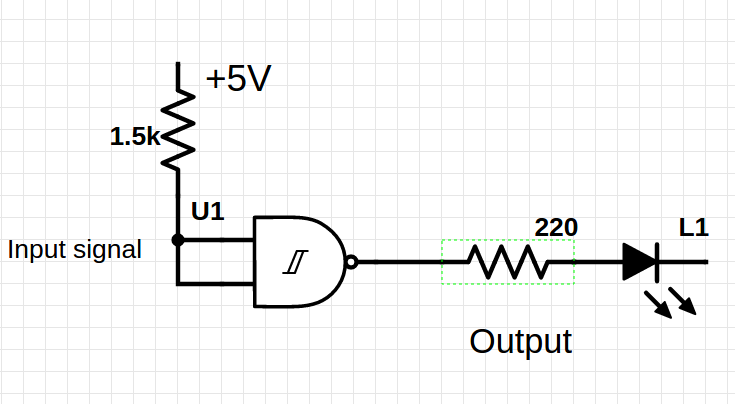
\includegraphics[scale=0.5]{images/transmitter_ckt_diag}
  \caption{Transmitter Circut PCB, Note : 1.5k connected to 5V}
  \label{fig:tx_circuit}
\end{figure}
\subsubsection{The receiver circuit}
\begin{figure}[h]
  \centering
  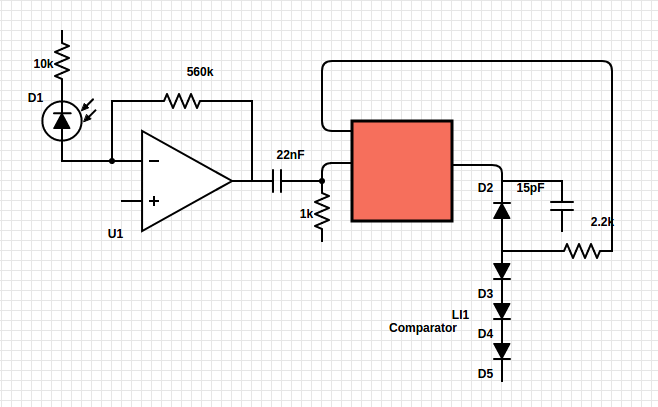
\includegraphics[scale=0.5]{images/receiver_ckt_diag}
  \caption{Receiver Circuit PCB. Note : 10K connected to 5V}
  \label{fig:rx_circuit}
\end{figure}
The first part of the consists of the photodiode which converts the light falling onto into electrical signals, The requirements of the photodiode was a quick response time, a spectral sensitivity in the visible spectrum and a large radiant sensitive area. The size of the
radiant sensitive area is crucial and therefore the photodiode used was a VISHAY BPW34. The spectral bandwidth is from 430 nm to 1100 nm and gives a perfect range for the intended application. It has a linear light intensity to current ratio and the radiant sensitive area is $7.5 \text{mm}^2$ , which was larger than most photodiodes found. It has a rise
and fall time of 100 ns each, which provides a switching frequency of $5 MHz$. This was enough since it is above the capabilities of the rest of the hardware and software.

This was followed a high gain voltage follower to convert the signal into a voltage waveform and also electrically isolate it from the rest of the circuit. For this, a OPAMP based voltage follower was used with a feedback resistance of $560 k \Omega$ to ensure a high gain. Such a high gain is required because the output of the photodiode is of the order of microamperes. The value of the resistance was chosen to ensure that the output was roughly in the range of 0-5 V. The value was chosen by trial and error mainly because the datasheet does not specify the typical values of current in the frequency range of interest. The OPAMP used was TL082. The requirements of the OPAMP in such case was to have a high slew rate so that the output is distorted to a minimum level because of the frequency response of the OPAMP, a low rise and fall time so that it quickly reacts to the input waveform. TL082 with a slew rate of $13 V\mu s$ and rise  seemed to be the ideal choice.

The output is then passed through a high pass filter made by using simple passive RC components. The specification of the filter design were stop frequency $ = 100 Hz$ and pass frequency $ = 5 kHz $. As a result, the transition frequency was chosen to be $ 700 Hz $ which is close to the geometric mean of the two and time constant of the circuit was designed to correspond to this frequency i.e., $ \dfrac{1}{RC} = 2 \pi \times 700 $. Using a standard value of capacitor $ =  22 nF $ we get the resistor value to be $ 10 k \Omega $. Using these values, a frequency response was plotted separately and checked. Here it is important to note that the capacitor serves dual purpose. Apart from the filter part, it also serves as a decoupling capacitor. The waveform until now was in the range of $ 0-5 \  V $ because the NAND gate switches between $0$ and $5$ V. After the capacitor the DC value of the system goes to $0$ and the voltage swings equally in the positive and the negative values.

The next element was a comparator. Here an OPAMP based comparator was not sufficient because it does not perform well in the high frequency range and hence a special comparator IC was used. The specifications of the comparator should have been to reach upto $ 750 kHz $ without distortion. LM 361 has a maximum delay of $20 ns$ and hence more than meets the specifications and is ideal for the purpose.

\subsubsection{Differentiator Circuit}
\begin{figure}[h]
  \centering
  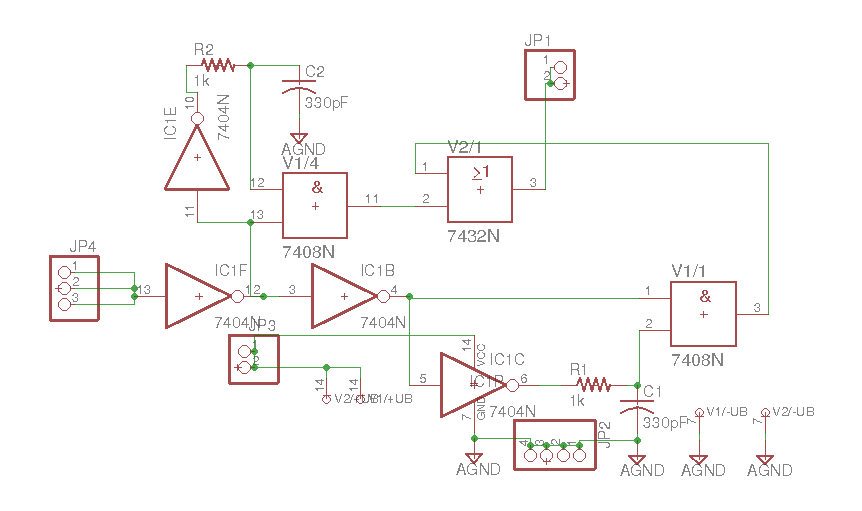
\includegraphics[scale=0.5]{images/Diff_sch}
  \caption{Differentiator PCB}
  \label{fig:Differentitor_circuit}
\end{figure}
The differentiator circuit, which is used for providing pulses at the edges of the input signal is implemented by basic logic gates - AND, OR and NOT and a delay circuit using a resistor and capacitor. To get pulses at positive edge of a signal $S_o$, it is first passed through a NOT gate to give a signal $\bar{S_o}$. The signal $\bar{S_o}$ is later passed through a delay circuit to give a delayed signal $S_1$. The AND of $S_1$ and $S_0$ gives the required pulse at the positive edge of the signal $S_0$. To get a pulse at the negative edge of $S_0$, a NOT of $S_0$ is taken initially and the exact same procedure as above is followed. Finally, ORing the pulses obtained gives the desired signal which corresponds to pulses outputted at the transitions of the input signal $S_0$.    

\subsubsection{PLL Circuit}
\begin{figure}[h]
  \centering
  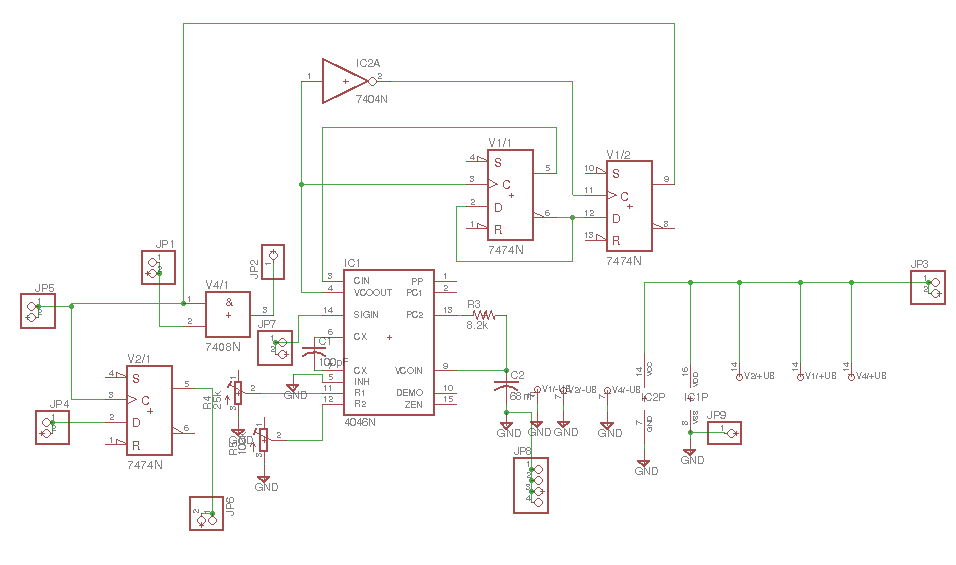
\includegraphics[scale=0.5]{images/PLL_sch}
  \caption{PLL pcb}
\end{figure}

The PLL circuit has already been discussed in great detail above in order to understand the working of the Data Synchronisation and Decoding circuit. The circuit consists of the IC CD4046B, which is essentially a PLL IC consisting of a two Phase Comparators, a tunable Low Pass Filter and a VCO circuit. Phase Comparator II has been used in the implementation of the project because of reasons mentioned in the earlier section. The Low Pass filter circuit can be tuned with the help of $R_3$ and $C_2$ as shown in figure *. Similarly, the lock range of the PLL can be determined with the help of $R_1$, $R_2$ and $C_1$ using the graph given in figure *. Potentiometer are used instead of $R_1$, $R_2$ which give an additional flexibility of altering the lock range. SN 7474 ICs have been used in order to implement the flip flops, namely $FF_1$, $FF_2$ and $FF_3$. NOT gates and AND gates shown in the figure * are implemented using the standard ICs 7404 and 7408 respectively. 


\subsection{Test Results}
The following tests were conducted to verify the individual components of the complete circuit.
\subsubsection{Transmitter circuit}
The circuit was not complicated and hence a simple test was conducted to ensure that the output follows the input without any phase difference. The output was voltage on the pin that was driving the LED.
\subsubsection{Receiver circuit}
Again for this circuit a simple point by point debugging method was employed. Since the current at the output of the photodiode is very low and not measurable by simple lab instruments like DMM hence directly the voltage after passing it through a large resistor was measured. Then specifically the working of the voltage buffer was tested.

All the tests upto this point were conducted by sending a pattern of alternating 0s and 1s via transmitter which had been tested previously. The output at this point is slightly distorted wave of high frequency modulated over a wave of very low frequency which is essentially the 50Hz noise due to ambient light. To filter out this noise, we pass this through a high pass filter and we find that the wave becomes stable with a zero DC value.

However, the wave is distorted due to imperfect frequency response of the OPAMP and the channel. The waveform is input to the comparator. To test this out we ensured that the comparator was giving the correct output and the zeros of the distorted waveform and output of the comparator matched. This is essential because it ensures that the bit width is not affected and there is no phase lag either. Also for the shift register, the output of each pin was checked on the DSO to ensure its proper working.

This is how we implemented a simple and effective point by point debugging method for the receiver circuit.


\subsubsection{Clock Synchronization and Data Recovery Circuit}
Since this is the most complex circuit as a whole, step-by-step testing was unavoidable.
\begin{enumerate}[label=(\alph*)]
\item \textbf{Testing of the Differentiator}\\ A square wave was given at the input of the Differentiator circuit, and verification of the working was done by observing whether pulses were seen at the transitions of the square wave 
\item \textbf{Testing of the VCO}\\ According to the figure shown below, appropriate values of R1,R2 and C1 need to be chosen in order to determine the lock/capture range of the PLL. To test that the lock/capture range was set as desired, the input of VCO, pin 9 of PLL was grounded in order to get the minimum frequency and later set High in order to get the maximum frequency and thus, the entire lock/frequency range.
    \begin{figure}[h]
    % \centering
    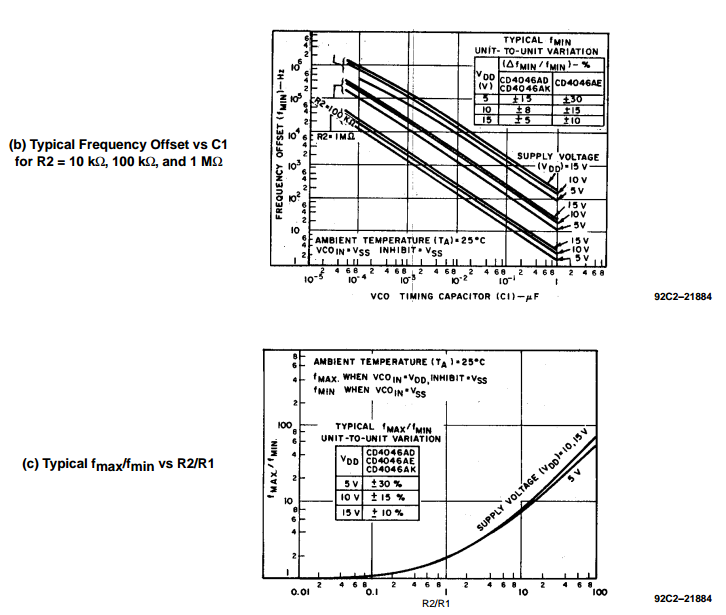
\includegraphics[scale=0.45]{images/FreqDeterm}
    \caption{Lock Range Determining Graphs}
    \label{fig:PLL}
  \end{figure}
\item \textbf{Testing of the PLL on Square Inputs}\\ In order to test only the PLL circuit, without the flip flops, a signal of frequency within the lock/capture range, was given at the input of PLL, the VCO output was shorted with the Comparator signal input to see whether the PLL locked on simple signals.
\item \textbf{Testing the PLL Circuit with Flip Flops}\\ The Entire PLL circuit, without the Differentiator and Decoder was tested next. Instead the output of AND Gate, again a square signal was given to the input pin 14 of PLL. Verification was done whether signal C and signal D were obtained as desired according to figure *
  %%%%%%%%%%%%%%%%%%%%%%%%%%%%%%%%%%%%%%% PICTURE%%%%%%%%%%%%%%%%%%%%%%%%%%%%%

\item \textbf{Testing the PLL Circuit along with Differentiator and  Encoder} \\ Finally, entire circuit connected in order to form a closed loop. A square pulse followed by a psuedo random sequence was given at the input of the differentiator and signals corresponding to B, C, D were observed. Expected desired observations confirmed the working of the clock synchronisation and Data recovery circuit.
\end{enumerate}

% \subsubsection{Software Testing}
\subsubsection{Transmitter code}
\begin{itemize}
\item \textbf{Transmitting wave}\\
  The transmitting waveform was initially tested by seeing the waveform of the output pins on the DSO. The waveform was stabilised and hence it was concluded that the Timer Interrupt is working correctly. Also the bits were manually calculated so as to cross check that the input data was correctly encoded. 
\item \textbf{Synchronization Sequnce Wave}\\
  Since the transmitter initially sent a stream of 0s which manchester encoded gave a stream of 01, it was important to check if the synchrnoizing sequence and the data sequnce was being sent at the same freqeuncy. This turned out to be a very big bug in our project, as the two were different.
\end{itemize}

\subsubsection{Receiver Code}
\begin{itemize}
\item \textbf{Hardware Breakpoints}\\
  Many Hardware breakpoints were used to determine the sources of error. Most of them were logical errors, and it was debugged only thanks to the almighty CCS.
\item \textbf{Data Reception}\\
  The most obvious and direct method of testing for receiver code was used, which is to see the bit errors in the received data. A stream of alphabets and sentences from a file were sent and there was no error in the received data buffer.
\end{itemize}
% \item 
%  
\subsection{Problems faced}
 As in any engineering task, we also faced a number of issues during the course of our project. The problem extended from design issues to the implementation specifics of the different parts of the hardware and software. 
\subsubsection{Hardware Problems}
 \begin{enumerate}
\item One of the initial problems faced initially was with the driver circuit. Initially, the LED was driven using an inverter, 7404. The problem was that when the output had to be driven high, the impedance of the PMOS used to drive the voltage was high and hence was distorting the waveform.
\item Initially for the high pass filter, a fifth order circuit was employed with a cut off of 10kHz. This was affecting the performance of the receiver circuit. This was because of the two additional OPAMP being introduced which were affecting frequency response of the circuit in the high frequency range because of their natural response. Hence as a solution to this, a simple RC filter design was adopted and integrated into the system.
\item \textbf{Differentiator}:
  \begin{itemize}
  \item This part of the circuit caused a lot of issued in implementation aspect. Initially, an OPAmp based differentiator was designed, however, it gave very thin pulses on the edges and of opposite signs on the different edges. An attempt was made to rectify the same using a diode rectifier which didn’t quite give the required results probably due to the capacitive effects of the diode.
  \item Next, another implementation was tried by passing a signal and its delayed version through an AND gate. The delay was obtained by using a NOT gate. However, this circuit failed again, much owing to thin pulses due to very short delay because of NOT gate and it also had another issue that it gave pulses only on the rising edge of the pulse.
  \item To counter the delay issue, an RC delay was added to increase the width of the pulse. And to add the negative edges also, the signal was passed through a NOT gate and procedure was repeated and the net signal was obtained by an OR of the two signals.
  \item This had couple of other issues. One, that size of the pulses was not equal on both the edges, which had been solved by using the OR of signal and its NOT. The second was that the amplitude of the pulses on the negative and positive edges were different and was rectified by passing the signal with lower amplitude by two NOT gates.
  \end{itemize}
\item \textbf{PLL}
  \begin{itemize}
  \item This was an issue faced in the initial stages of designing a PLL circuit. Initially the input to the PLL circuit had a zero DC bias and the waveform was swinging between $-2 V$ and $ 2 V$. However, it was later realised that the PLL did not work for such signals. Nowhere this caution was mentioned in the documents that had been referred. For this purpose, the voltages at the comparator were changed to ensure that the output is between $0$ and $5 V$.
  \item Another issue was faced was during the integration of the hardware and software. The PLL circuit had been designed and tested independently and had been locking with the clock. To try for arbitrary sequences the input had to be taken from a tivaC which would send a synchronising pulse followed by an arbitrary pulse. It was found that PLL was not locking wherein it was supposed to. After a lot of debugging, it was realised that even if the arbitrary sequence was a sequence of alternating $1$s and $0$s, the PLL was not getting locked. Further, it was realised that the frequency at which the tiva was sending the synchronisation pulse and the arbitrary sequence were different because they had been called from different functions which took different amounts of time to be executed. This software bug was resolved by making it the same function and which then ensured that the PLL locked even on arbitrary sequences.
  \end{itemize}
\end{enumerate}

\subsubsection{Software Problems}
\begin{enumerate}
\item \textbf{Initial Steep Learning Curve for CCS}\\
  CCS is slightly advanced and it is daunting to learn how exaclty to use CCS. It took around 1 week to successfully setup CCSv7 and get everything to work. There were added hindrances in TivaC, which is initially not recognised as an USB device by the PC, and its vendor id and device id need to be manually added to the operating system to recognise it as a USB device.
\item \textbf{Code for USB Transmission}\\
  The main problem with USB link faced was that there is a garbage value of about 30 bytes between the PC and the device. Moreover it takes a significant amount of time to setup (3-4 seconds, note: compared to the processor speed). The main disadvantage of USB is that the speed of USB transmission is extremely less than that of the visible light Communication link. Moreover there a significant number of function calls that need to be made to setup a successful USB connection. This too took a lot of time to debug.
\item \textbf{SysCtlGetClock() returns incorrect result}\\
  When operating TivaC at 80MHz, it is found that SysCtlGetClock() which should return the processor clock rate, gives erroneous output. This is a known bug in CCS. This means that even though the system might work when it run via CCS, once it is reset, the working breaks down. For our case, the Transmission rate went from 100kHz to 236kHz on resetting the pin. Instead of calling this function, this value needs to be hardcoded while operating at 80MHz.
\item \textbf{Dual Functionalities of GPIO Pins}\\
  Many gpio pins have dual functionalities. For example the pin PB3 is also used for USBStdio communication, and it was being used for sending the data, and hence the waveform that resulted didn't get stabilised. Before using any gpio pin, it must be carefully checked if that pinhas any other functionality.
\item \textbf{Multiple Interrupts being called at the same time}\\
  Extra care must be taken to ensure that multiple interrupts are not called at the same time. If this is required to happen the priority order must be checked first. For testing purposes, both reception and transmission code were run on the same tivaC board, which resulted in occurence of a gpio interrupt due to receiver in between a timer interrupt of the transmittter. 
\item \textbf{Fault ISR}\\
  This is perhaps the most common bug in any code. Many a times for no apparent reason the code stops at FaultISR interrupt. This basically happens when the software is stuck in an infinite loop. But most often than not (atleast in our experience) this was not the problem. The culprit was rather the out of array indexing, which basically means we were incorrectly trying to access some an element of an array out of its length. 
\end{enumerate}

\subsection{Final Product Images}
\begin{figure}[H]
  \centering
  \includegraphics[scale=0.05]{images/diff_pll}
  \caption{Differentiator and PLL pcb}
  \label{fig:diff_pll}
\end{figure}

\begin{figure}[H]
  \centering
  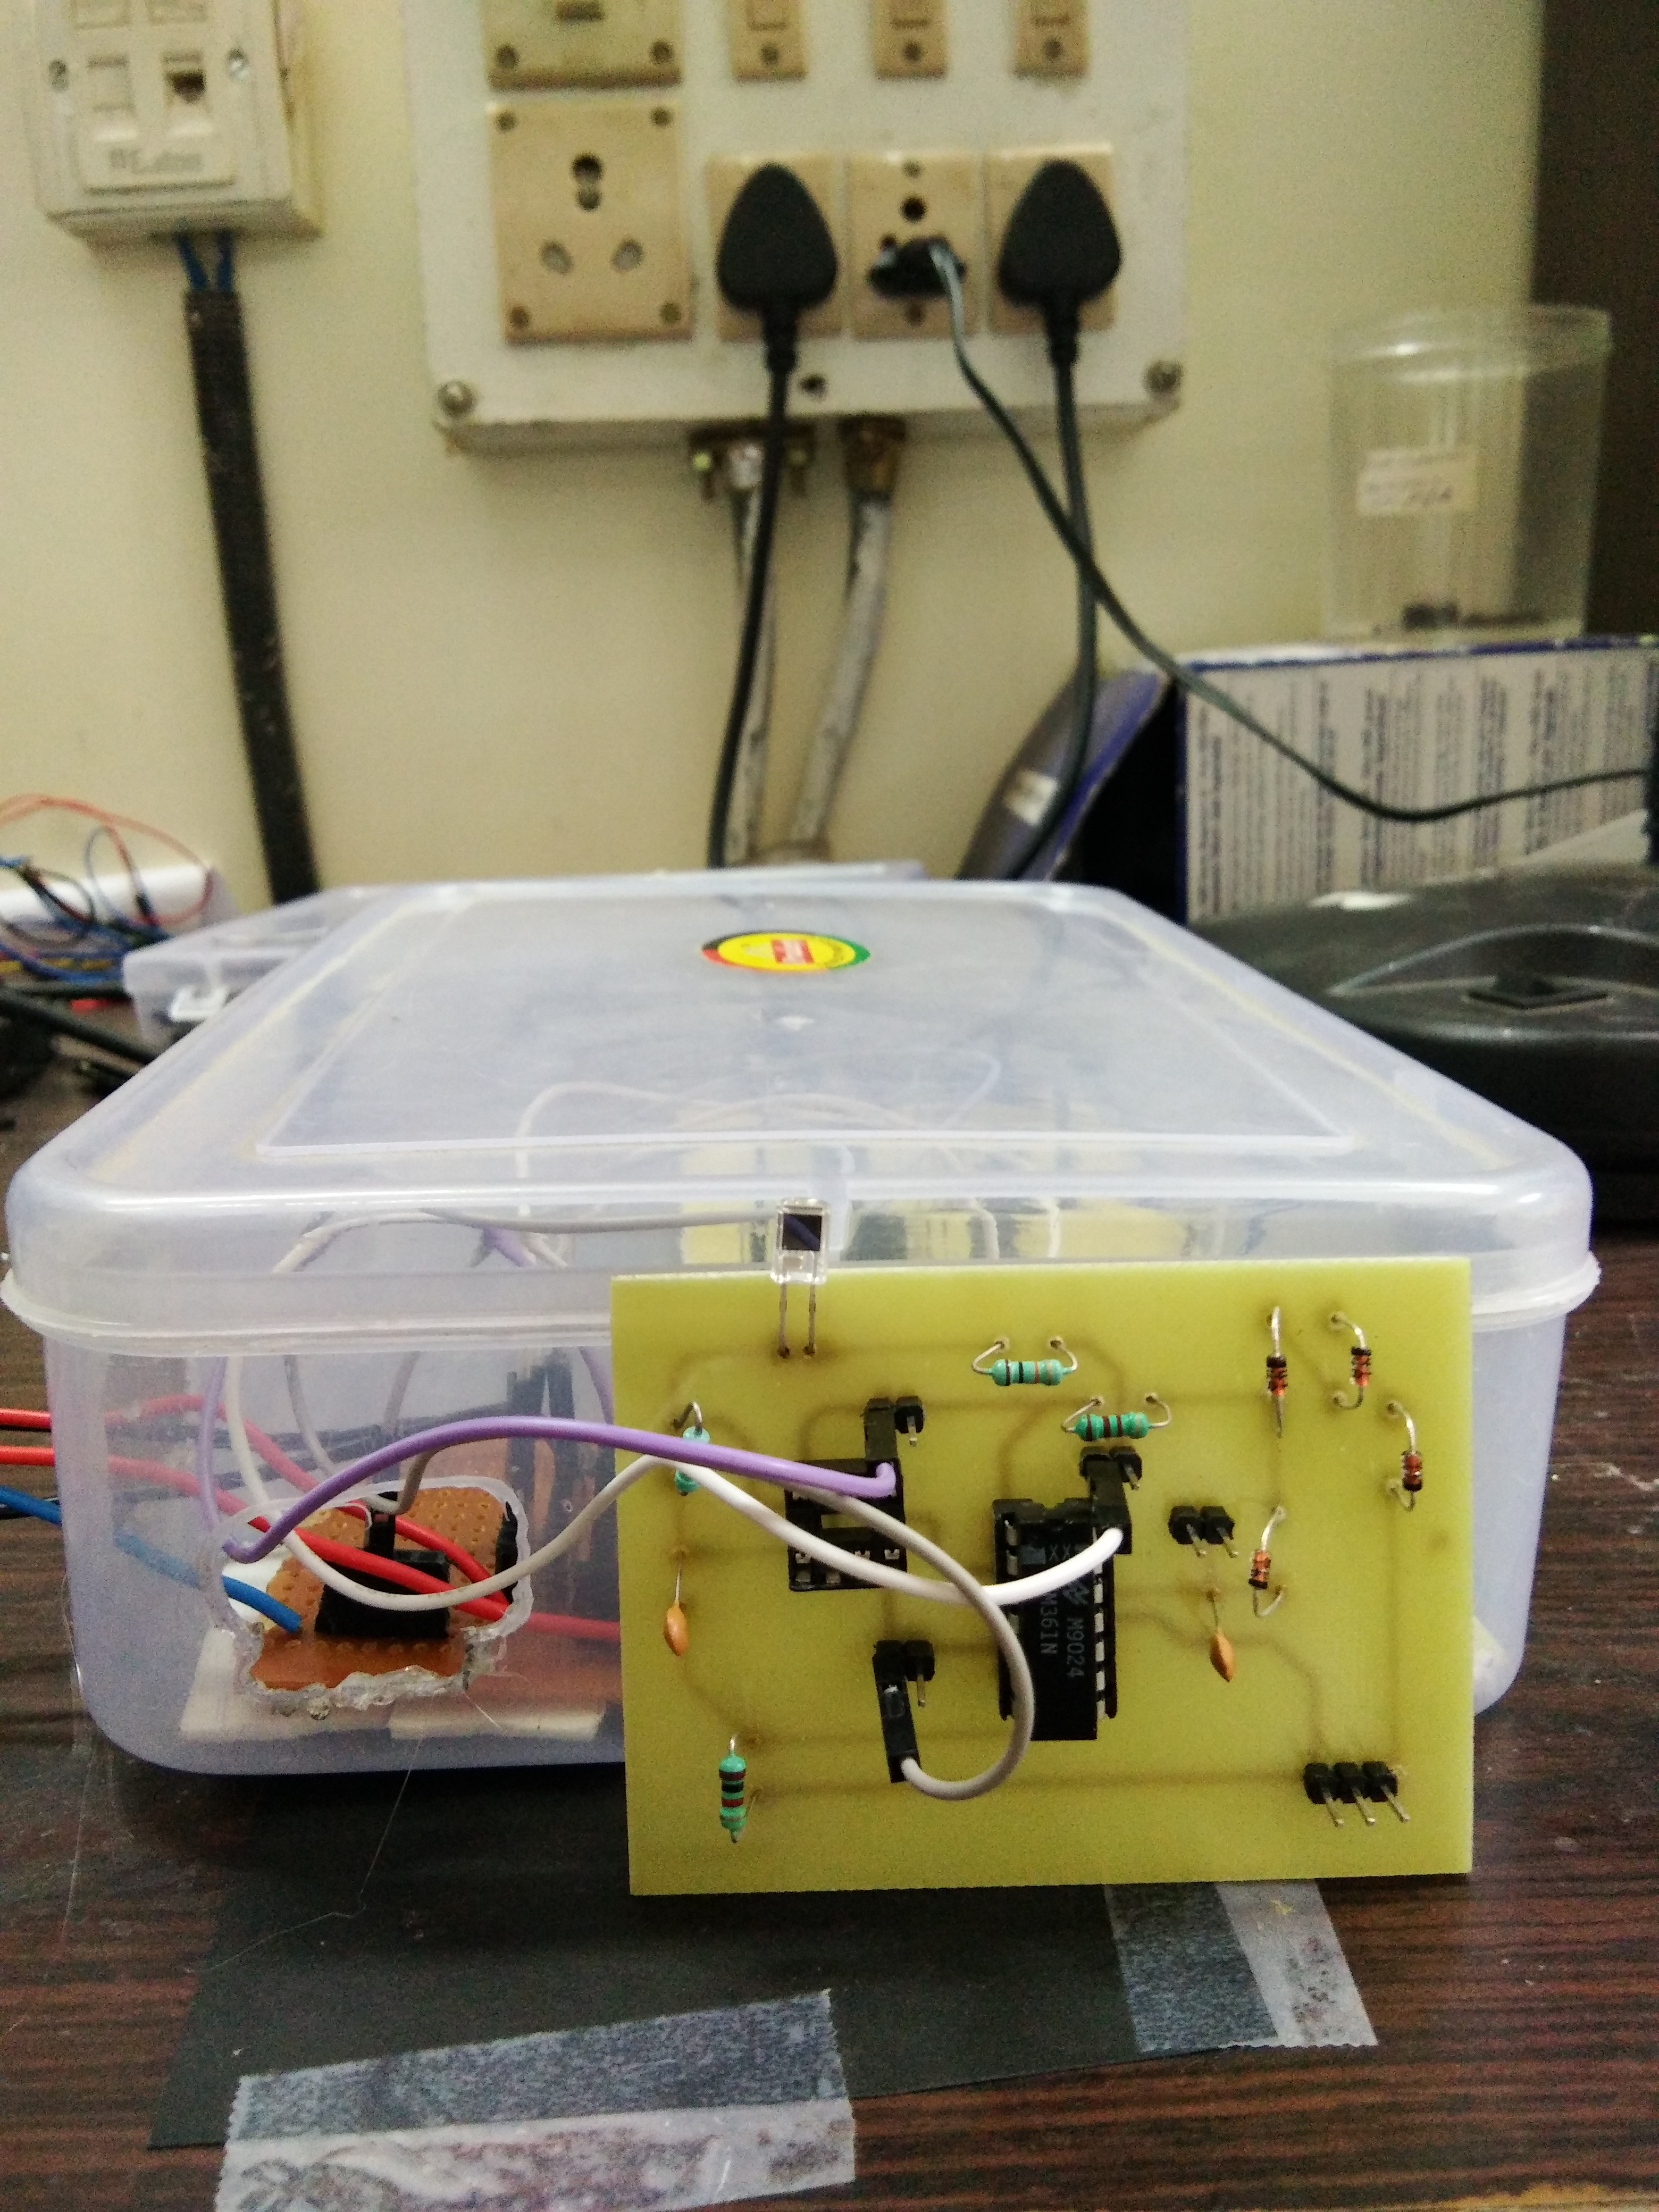
\includegraphics[scale=0.05]{images/receiver_box}
  \caption{Receiver in Box}
  \label{fig:rx_box}
\end{figure}
\section{Chapter 5 : Conclusion and suggestions for future work}

The project was finally completed, almost reaching the intended aims by the end of the semester. The system is fairly robust to ambient light and and provides speeds upto $300$ kbps with negligible bit error rate. A number of constraints in the system are because of the constraint of the hardware used and hence was not able to completely achieve the intended specifications. This project can be developed in future in the following domains:
\begin{enumerate}
\item The performance of the PLL IC currently employed begins to get affected near the range of $300$ kHz whicu puts a constraint on the time period of a transmitted bit and thus on the data rate. This issue can be worked upon by using a better but expensive PLL IC.
\item Another issue that limits the performance is the buffering of tivac. The tivac has a small and limited buffer which puts an upper cap on the amount of data that can be transmitted at once. A device with a larger buffer would help increase the overall effective data rate.Another thing that can be worked upon is a dynamic buffer. The buffer of tivac can either read data or transmit it. It can only do one at a time and cannot do both of them simultaneously. The employment of a device which facilitates this would be a huge boost to the performance of the system in terms of data rates.
\item The current implementation uses a torch as a light source. Another thing that is possible is to use an actual light source which has a primary purpose of illumination for the purpose of communication. This will be a great step in making this an actual deployable product. 
\end{enumerate}

\section{Chapter 6 : References}
\begin{enumerate}
\item Visible Light Communication by \textit{Shlomi Arnon}
\item TivaWareTM Peripheral Driver Library User's Guide by \textit{Texas Instruments}
\item Getting Started with the Tiva TM4C123G LaunchPad Workshop by \textit{Texas Instruments}
\item CD4046B Phase-Locked Loop: A Versatile Building Block for Micropower Digital and Analog Applications \textit{Texas Instruments}
\end{enumerate}

\end{document}

